%
\graphicspath{{figures/mva_bdt/}}
\subsubsection{Input variables}
\label{sec:BDT-input-variables}

BDT is trained for each mass point of Higgs boson $t\bar{t}H(\rightarrow t\bar{t})$ as signal and $t\bar{t}+$jets as background. 
All BDTs are using the same set of input variables, which are the variables retrieved from the SM$t\bar{t}t\bar{t}$ analysis plus some new variables that can improve the AUC performance. 
This section shows the 18 input variables used in the BDT for both 1L and OS channels.
The selected variables are divided into five groups based on different physics characteristics.

\begin{itemize}
\item \textbf{Global event activity in the transverse plan:}

$t\bar{t}H(\rightarrow t\bar{t})$ leads to more energetic and central activities than $t\bar{t}+$jets, especially the high mass Higgs boson signal.
Therefore the signal generally gives a larger value for the following variables than the $t\bar{t}+$jets background.
The heavier of BSM Higgs boson, the higher separation between the signal and background.

\begin{itemize}
\item The transverse momentum sum of all the reconstructed jets and leptons in the events ($H_{T}$)
\item Centrality of all reconstructed jets and leptons ($\sum_{i} {p_{T}}_{i} / \sum_{i} E_{i}$)  
\end{itemize}
\item \textbf{Jet activity:}

$t\bar{t}H(\rightarrow t\bar{t})$ generates more hard jets than $t\bar{t}+$jets.
The following variables get a boosted value in $t\bar{t}H(\rightarrow t\bar{t})$.

\begin{itemize}
\item Jet multiplicity ($N_{jets}$)
\item Transverse momentum of leading jet (${p_{T}}_{0}$)
\end{itemize}

The extra jets from $t\bar{t}+$jets are mainly from the radiation while high jet multiplicity is mainly come from the prompt particles in $t\bar{t}H(\rightarrow t\bar{t})$
The radiation jets highly affected the separation between jets and the invariant mass of jets with angular threshold.
The following variables are used to compare the radiation structure between signal and background.

\begin{itemize}
\item Average angular separation across all pairs of jets ($\Delta R^{avg}_{jj}$)
\item Invariant mass of the triplet jets with minimum angular separation~\footnote{The angular separation of triplet of jets is defined as $\Delta R_{ijk}=\sqrt{\Delta R^{2}_{ij}+\Delta R^{2}_{ik}+\Delta R^{2}_{jk}}$, where $i$, $j$ and $k$ are the indices of the three jets} ($M^{min. \Delta R}_{jjj}$)
\item Average invariant mass of all the jets triplets with angular separation smaller than three ($M^{\Delta R<3}_{jjj}$)
\end{itemize}

In 1L-channel, it is expected that four hard jets are directly come from top-quarks in $t\bar{t}$+jets, while the remaining jets are generally the soft radiation.
In contrast, ten hard jets are expected come from top-quarks in $t\bar{t}H(\rightarrow t\bar{t})$. 
The following variable shows the properties between first few leading hard jets and the remaining soft jets among $t\bar{t}H(\rightarrow t\bar{t})$ and $t\bar{t}$+jets.

\begin{itemize}
\item The ratio of transverse momentum sum of the first four leading jets to the transverse momentum sum of the remaining jets ($\sum^{3}_{i=0}{p_{T}}_{i} / \sum_{i\geq 4} {p_{T}}_{i}$)
\end{itemize}

\item \textbf{b-tagging information}

$t\bar{t}H(\rightarrow t\bar{t})$ generates more energetic b-jets with respective to $t\bar{t}+$jets, where extra b-tagged jets are come from radiation.
The energy of b-jets is higher in $t\bar{t}H(\rightarrow t\bar{t})$ with heavier Higgs boson.
The b-tagging working point used for these variables is defined as DL1r 70\%.
The following variables related with b-tagged jets properties give a separation between signal and background.

\begin{itemize}
\item Minimum angular separation among all pairs of b-tagged jets and leptons ($\Delta R^{min}_{bl}$)
\item Minimum angular separation among all pairs of b-tagged jets ($\Delta R^{min}_{bb}$)
\item Average invariant mass of all the b-tagged jets triplets ($M^{avg}_{bbb}$)
\item Minimum invariant mass of all pairs of b-tagged jets ($M^{min}_{bb}$)
\item Sum of the pseudo continuous b-tagged score of the four leading jets ranked in DL1r score ($\sum^{i<4}_{i=0} {pcb}_{i}$)
\end{itemize}

\item \textbf{RC-jets information}

$t\bar{t}H(\rightarrow t\bar{t})$ gets more jets activities in the transverse plan and some of the produced top-quarks could be boosted, especially for the heavy Higgs boson signal.
This boosted structure can be re-clustered into large-R jets with sub-structure that are not favour in $t\bar{t}+$jets.

\begin{itemize}
\item Number of RC-jets with a mass higher than 100 GeV ($N_{RC100}$)
\item Sum of the first $k_{T}$ splitting scale $d_{12}$ of all RC-jets ($\sum d_{12}$)~\footnote{The $k_{T}$ splitting scale $d_{ij}$ is defined as the recombination distance between the jets constituent from a $k_{t}$ algorithm: $d_{ij}=min({p_{T}}_{i}^{2},{p_{T}}_{j}^{2})\times \Delta R^{2}_{ij}$.}
\item Sum of the second $k_{T}$ splitting scale $d_{23}$ of all RC-jets ($\sum d_{23}$)
\end{itemize}

\item \textbf{Leptons and neutrino activities:}
The leptons are expected from the W-boson which is decayed from top-quark.
$t\bar{t}H(\rightarrow t\bar{t})$ generally leads to more energetic leptons and neutrinos (which is described in miss transverse momentum MET) than $t\bar{t}$+jets, especially for the heavy Higgs boson.
The following variables describe the leptonic activities of the events.

\begin{itemize}
\item Missing transverse momentum ($E^{miss}_{T}$)
\item W reconstructed transverse mass ($m_{T}(\ell,E^{miss}_{T})$) for 1L and the invariant mass of two leptons ($m_{\ell \ell}$) in OS.
\end{itemize}

\end{itemize} 

Several input variables distributions, with separation power defined as
%%%%Equation: Variable Separation%%%%
\begin{equation}
\mathrm{Sep}=\frac{1}{2}\sum_{\mathrm{bins}} \frac{(s-b)^{2}}{s+b}~,
\label{eqn:varSeparation}
\end{equation}
%%%%%%%%%%%%%%%%%%%%%%%%%%%%%%%%%%%%%%%
where $s$ and $b$ are the signal and background ($t\bar{t}+\mathrm{jets}$) yields respectively of each bin, are shown in Figure~\ref{fig:1L_inputVarDistribution} and the correlation between them are shown in Figure~\ref{fig:1L_inputVarCorrelation}.

%%%%%%%%%%%%%%%%%%%%%%%%%%%%%%%%%%%%%%%
where $s$ and $b$ are the signal and background ($t\bar{t}+\mathrm{jets}$) yields respectively of each bin. 

%%%%Fig: Input Variables Plots%%%%
\begin{figure}[!htp]
    \centering
    \begin{subfigure}[t]{0.32\textwidth}
        \centering
        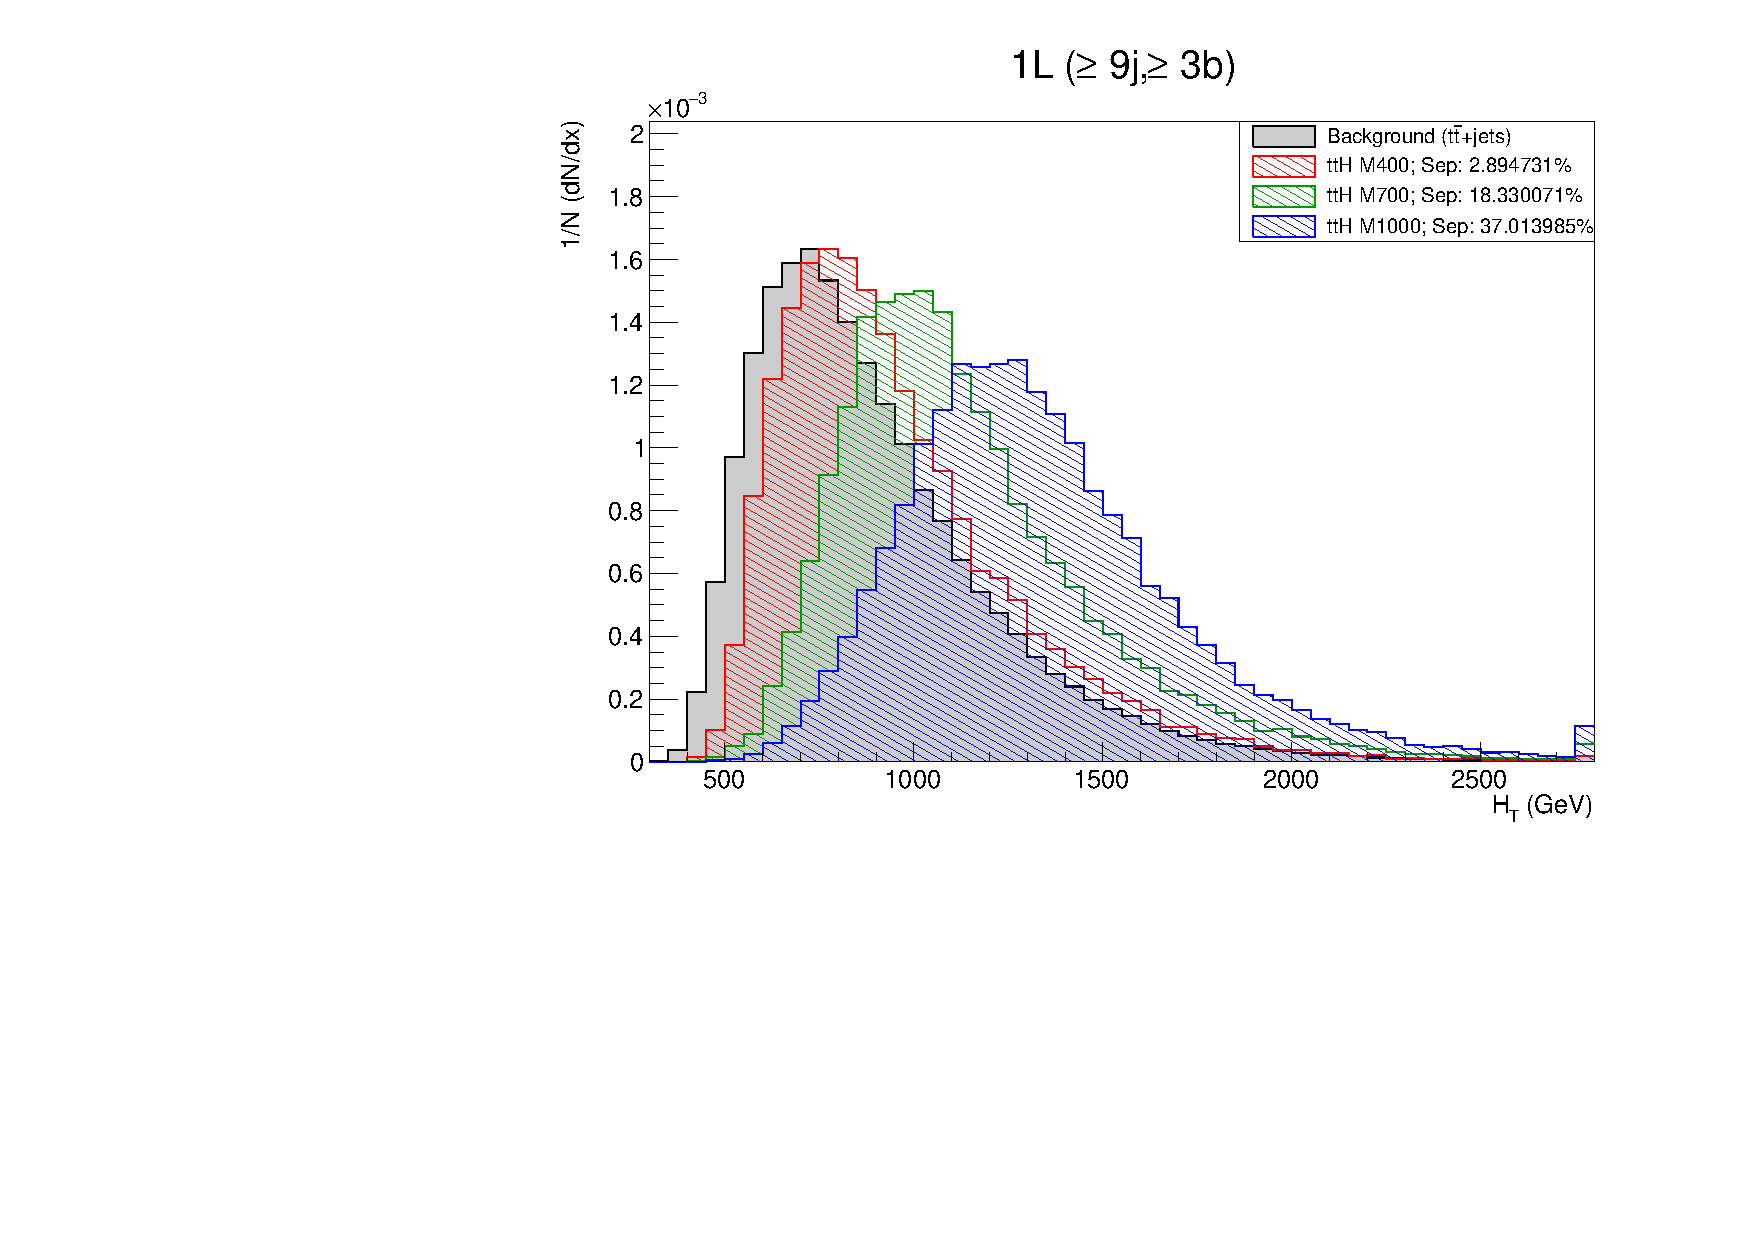
\includegraphics[width=\textwidth]{inputVar/1L/HT_all_ljets_ge9jge3b.pdf}
        \subcaption{$H_{T}$}
    \end{subfigure}
    \begin{subfigure}[t]{0.32\textwidth}
        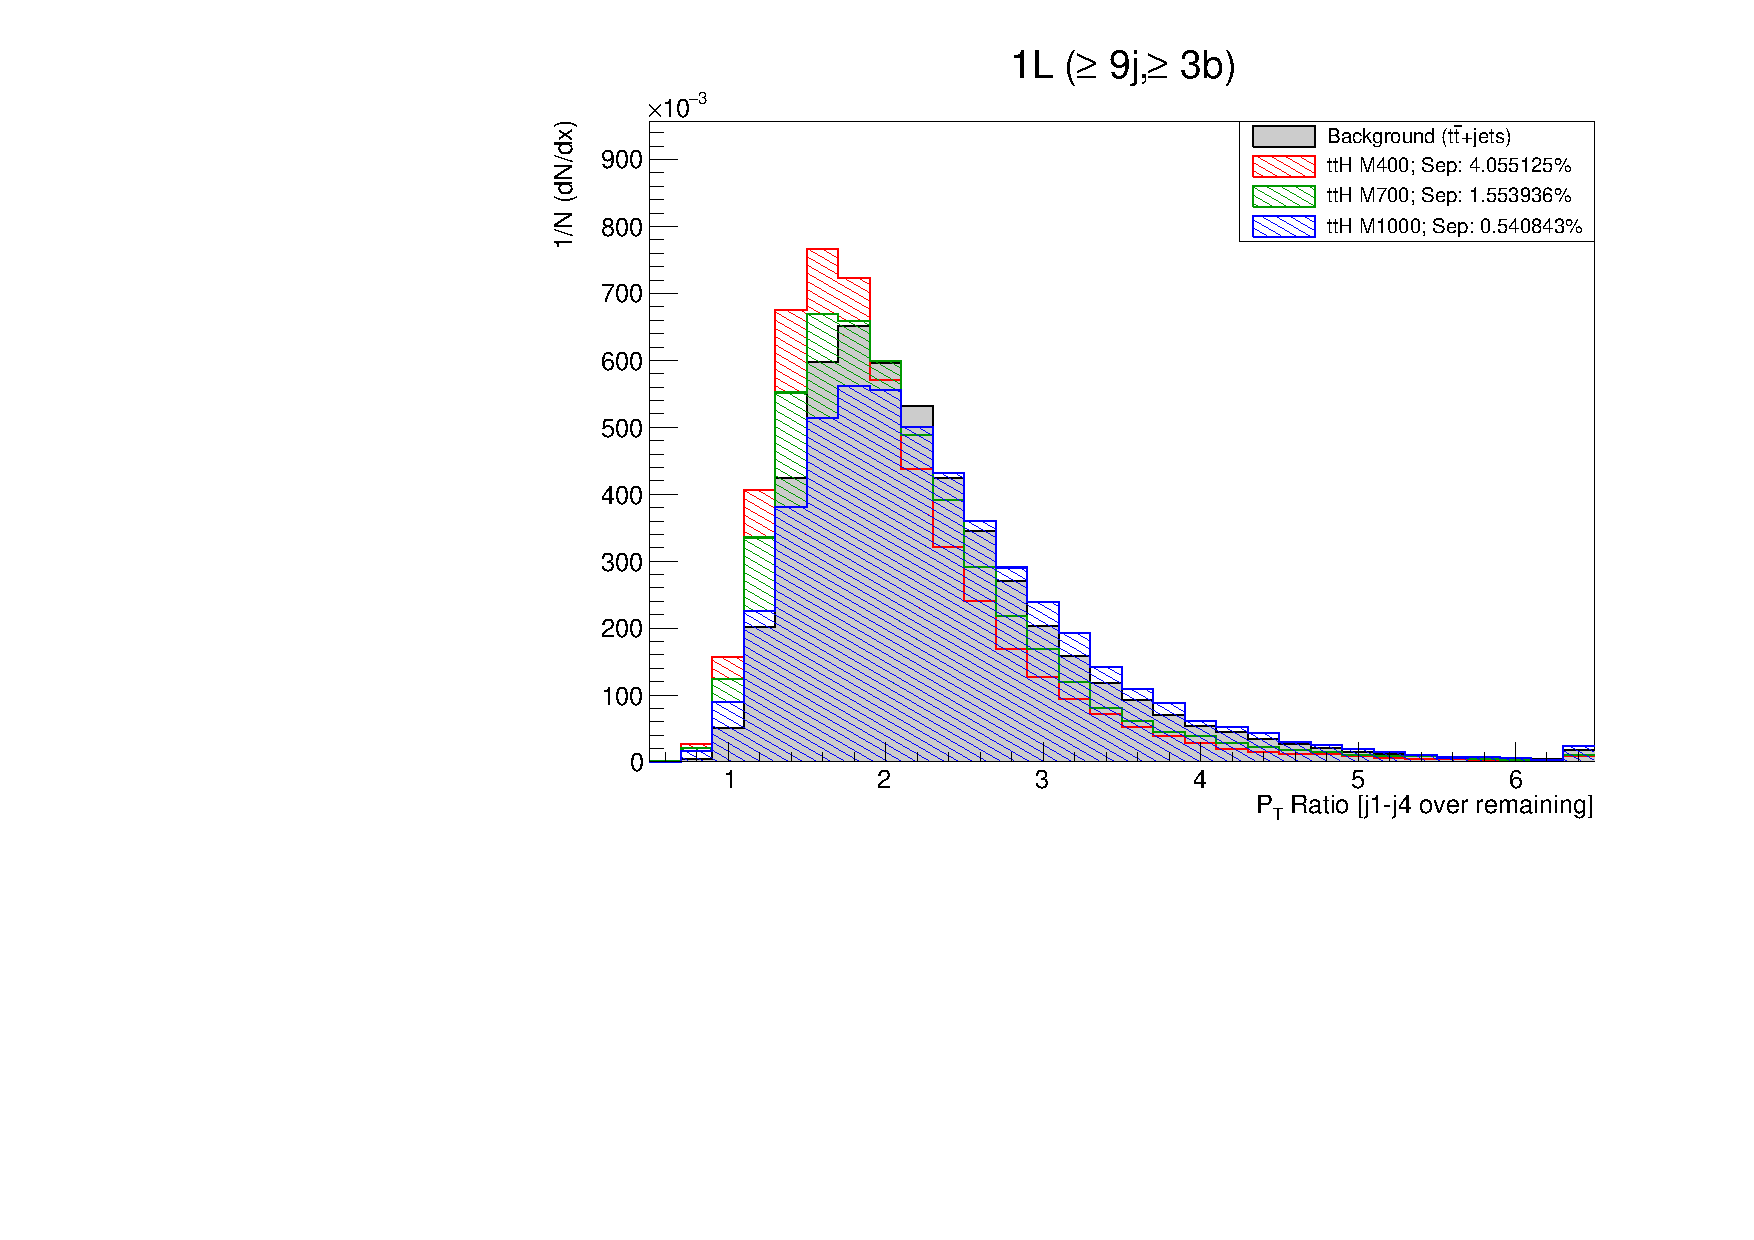
\includegraphics[width=\textwidth]{inputVar/1L/HT_rat_ljets_ge9jge3b.pdf}
        \subcaption{$\sum^{3}_{i=0}{p_{T}}_{i} / \sum_{i\geq 4} {p_{T}}_{i}$}
    \end{subfigure}
    \begin{subfigure}[t]{0.32\textwidth}
        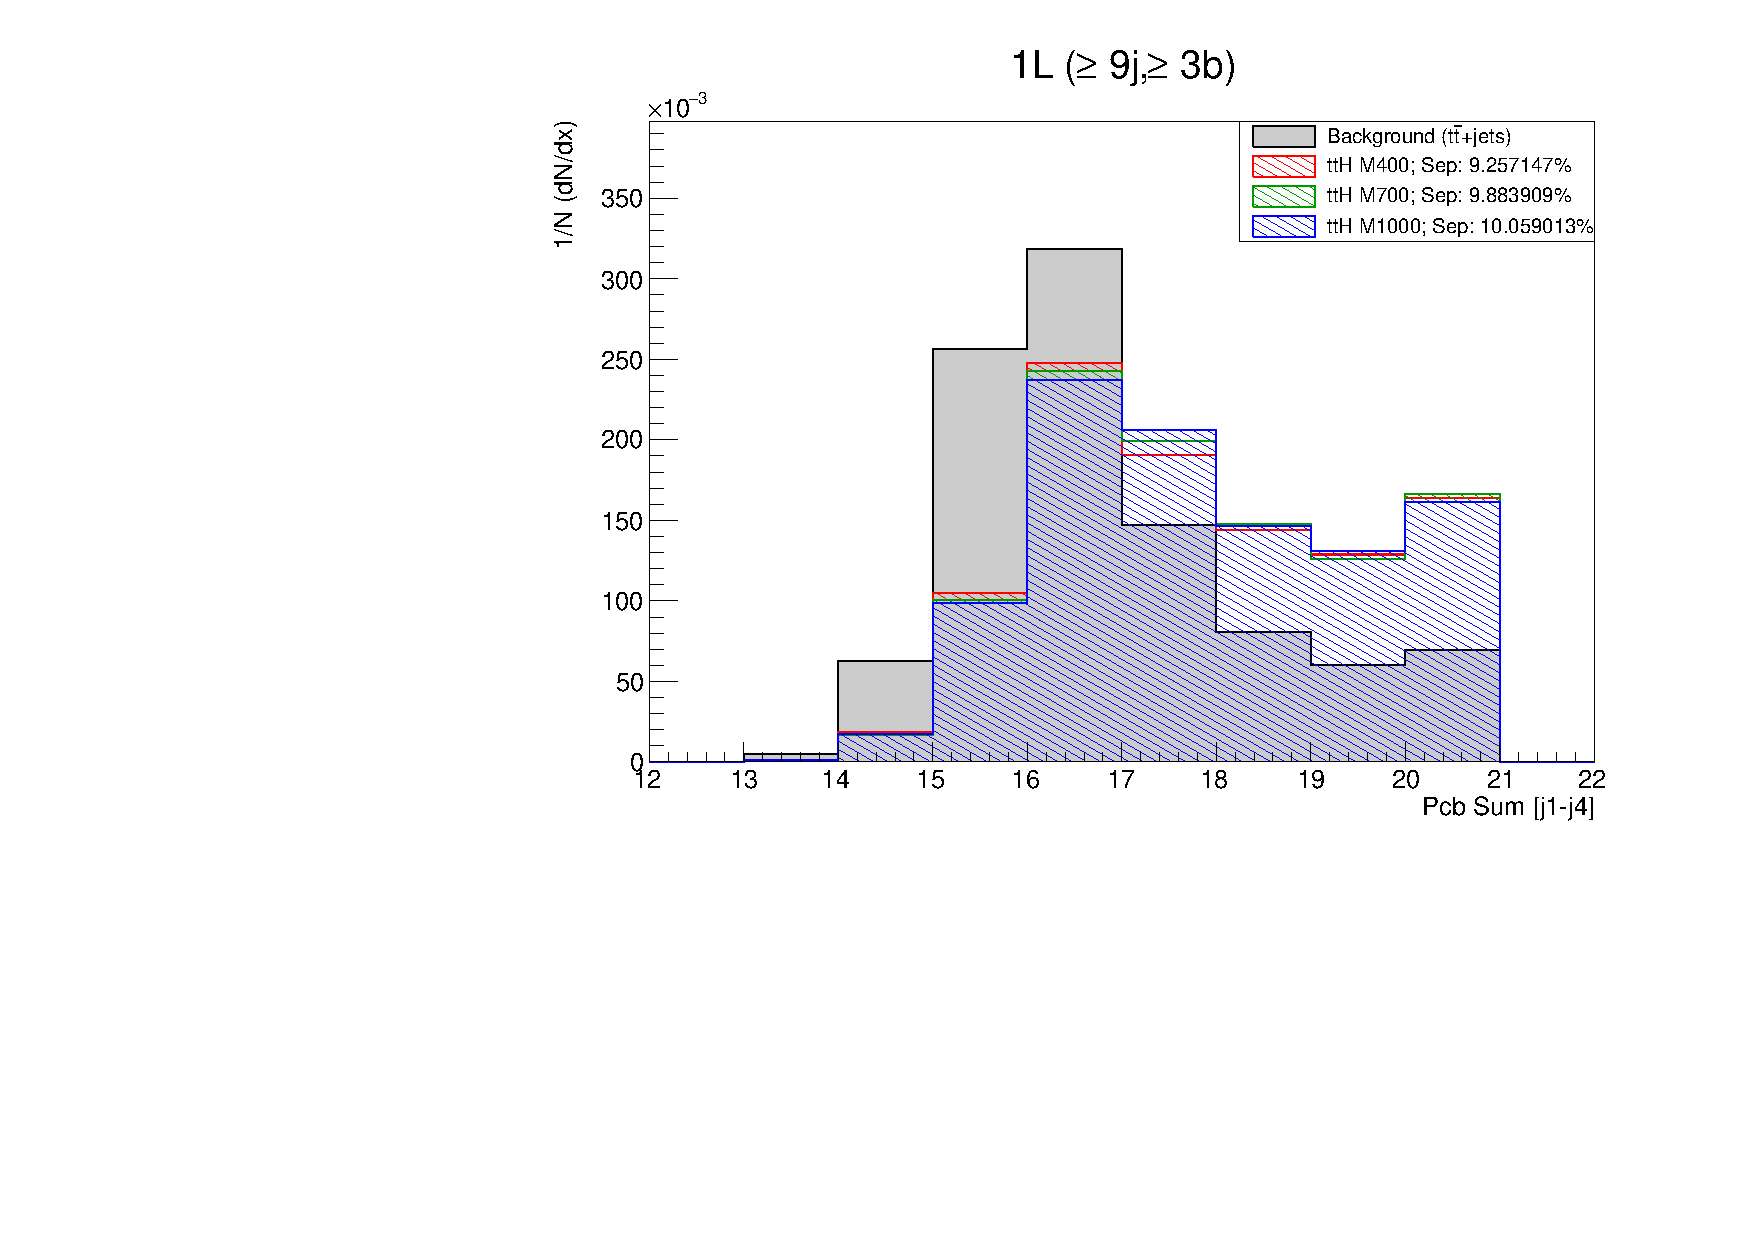
\includegraphics[width=\textwidth]{inputVar/1L/pcbSum_ljets_ge9jge3b.pdf}
        \subcaption{$\sum^{i<4}_{i=0} {pcb}_{i}$}
    \end{subfigure}
    \newline
    \begin{subfigure}[t]{0.49\textwidth}
        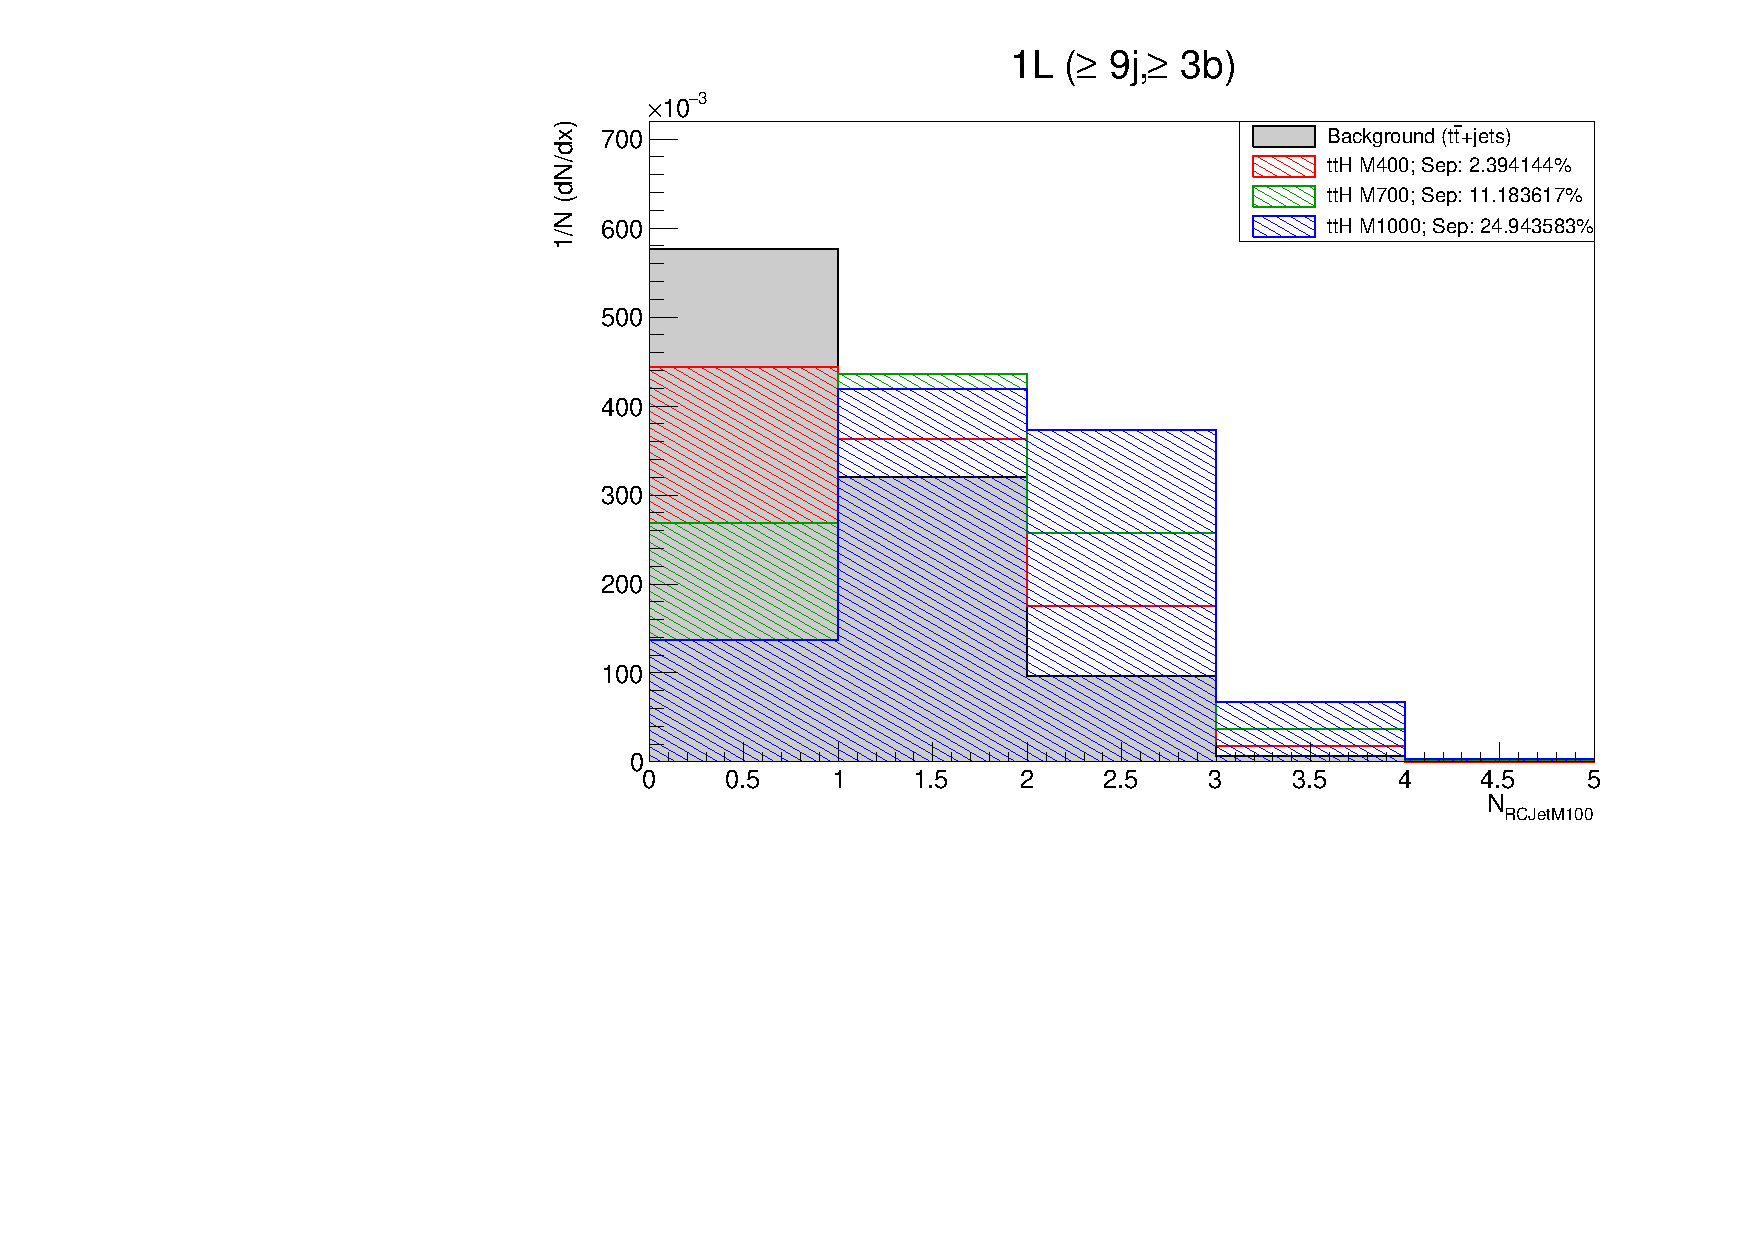
\includegraphics[width=\textwidth]{inputVar/1L/nRCJetsM100_ljets_ge9jge3b.pdf}
        \subcaption{$N_{RC100}$}
    \end{subfigure}
    \begin{subfigure}[t]{0.49\textwidth}
        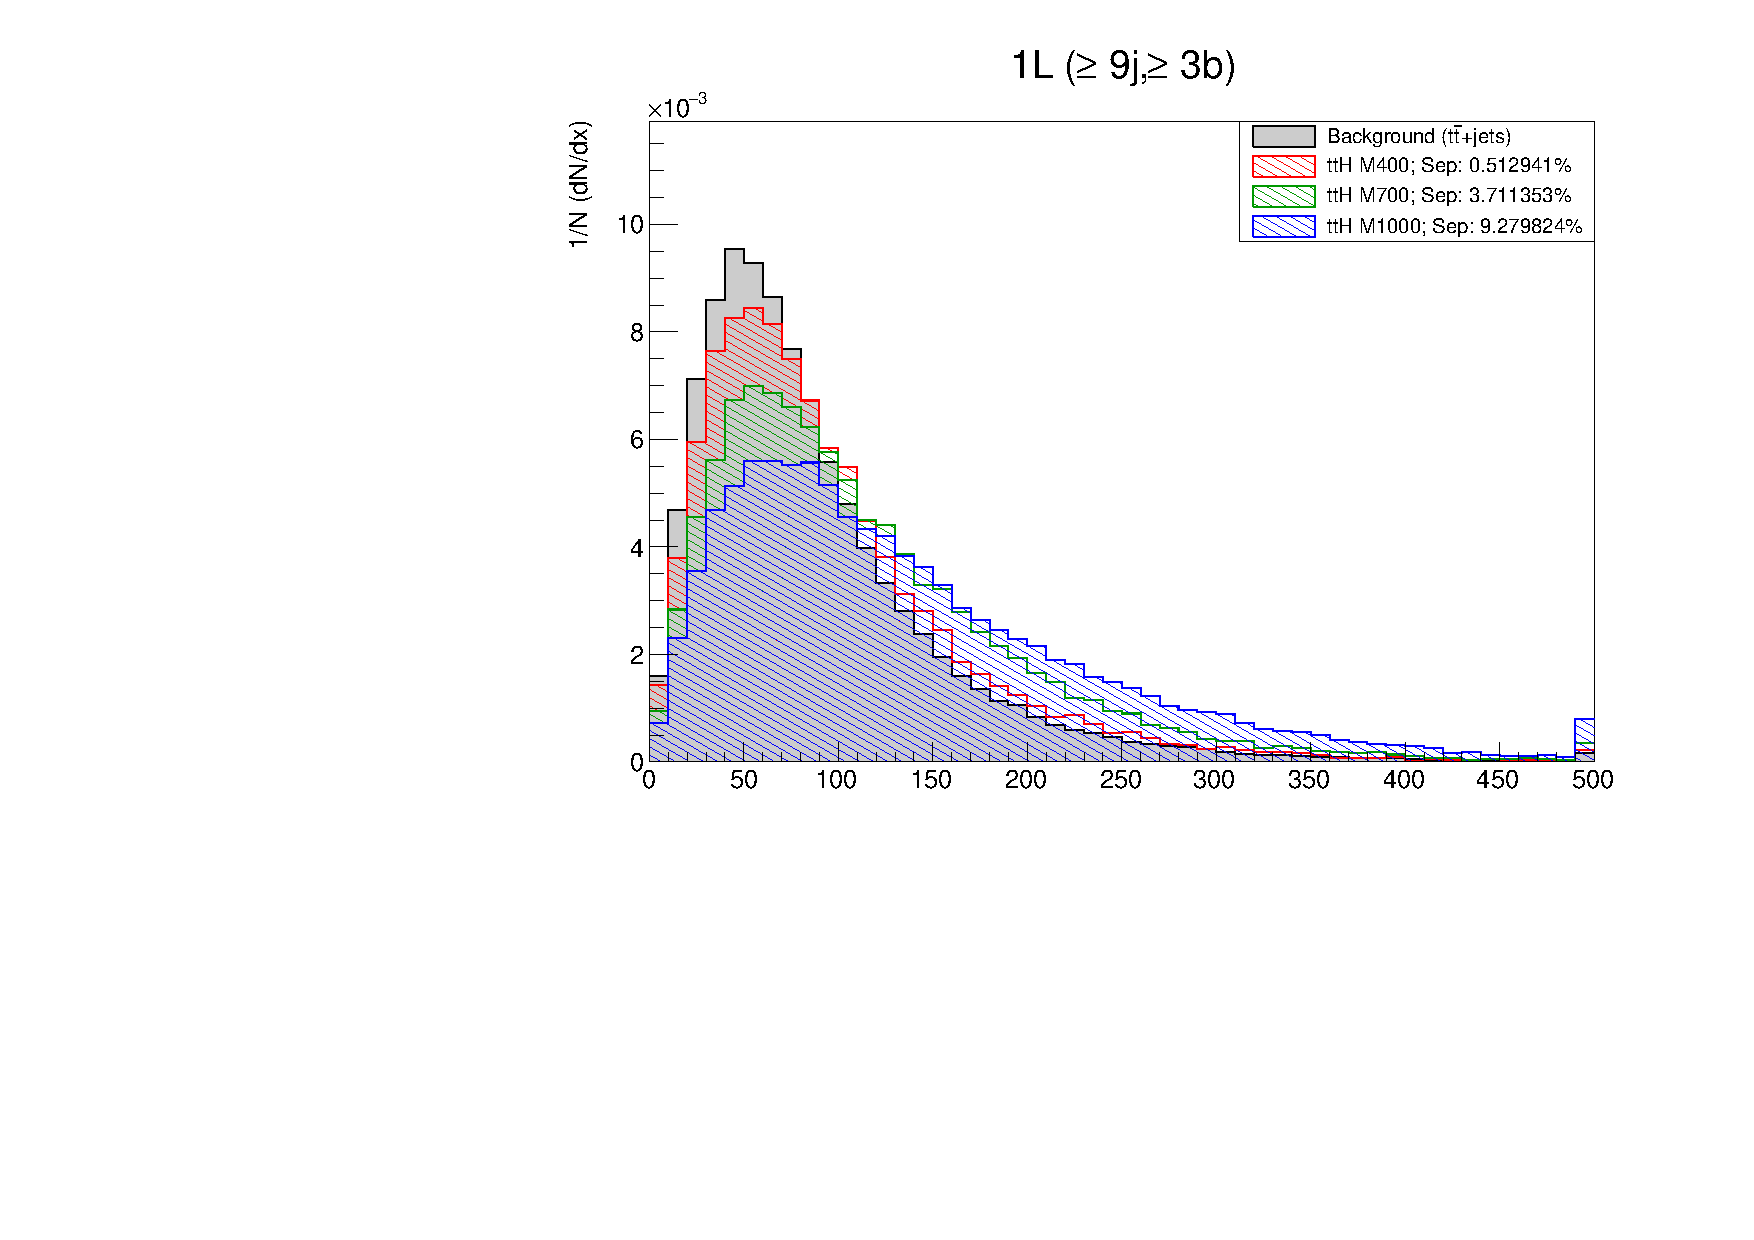
\includegraphics[width=\textwidth]{inputVar/1L/met_met_ljets_ge9jge3b.pdf}
        \subcaption{$E^{miss}_{T}$}
    \end{subfigure}
    \caption{\label{fig:1L_inputVarDistribution}Some input variables distribution of $t\bar{t}$+jets, and $t\bar{t}H(\rightarrow t\bar{t})$ with BSM Higgs boson mass of 400 GeV, 700 GeV and 1000 GeV in the region of $\geq9j \geq 3b$. The distributions are normalized to one.}
\end{figure}
%%%%%%%%

%%%% Fig: Input Variable Correlation %%%%
\begin{figure}[!htp]
    \centering
        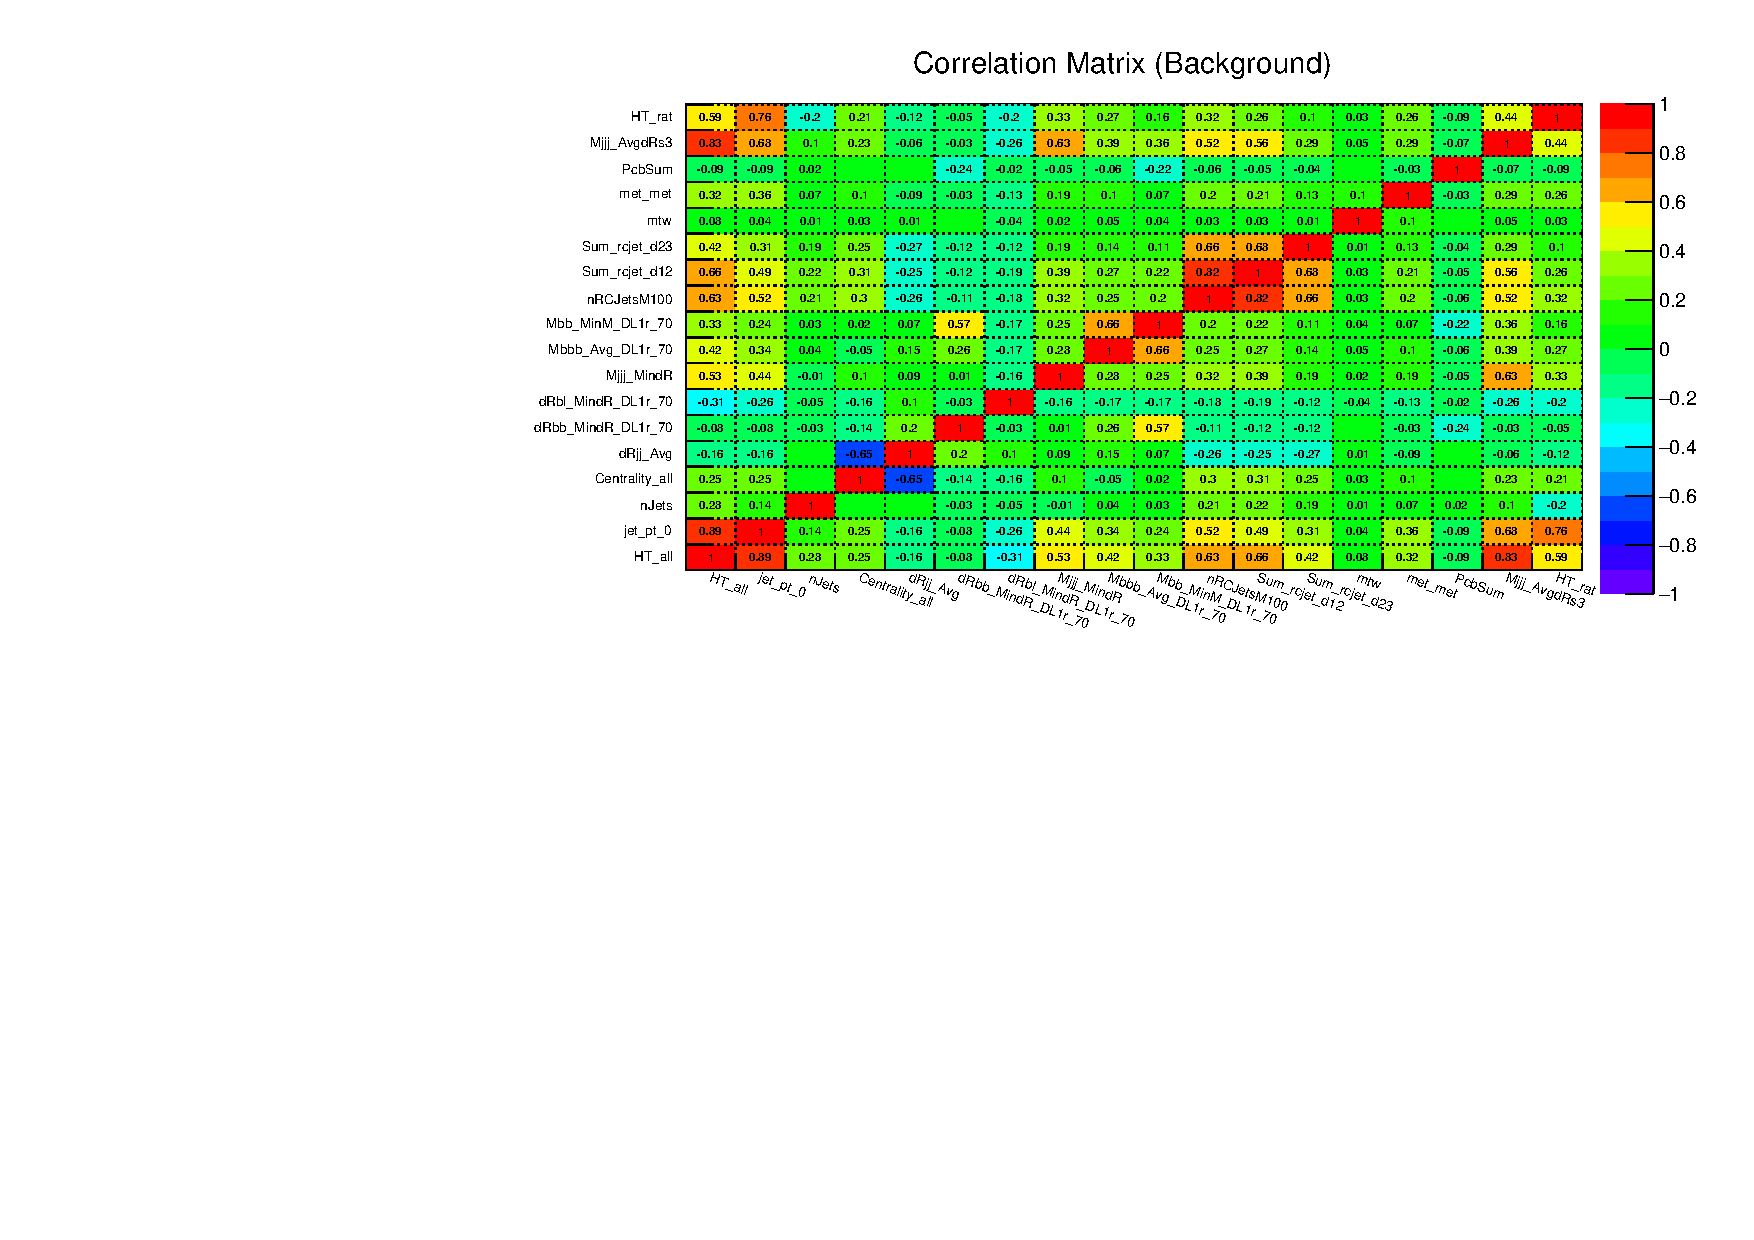
\includegraphics[width=0.55\textwidth]{inputVar_correlation/1L_correlation_ttbar.pdf}
    \newline
        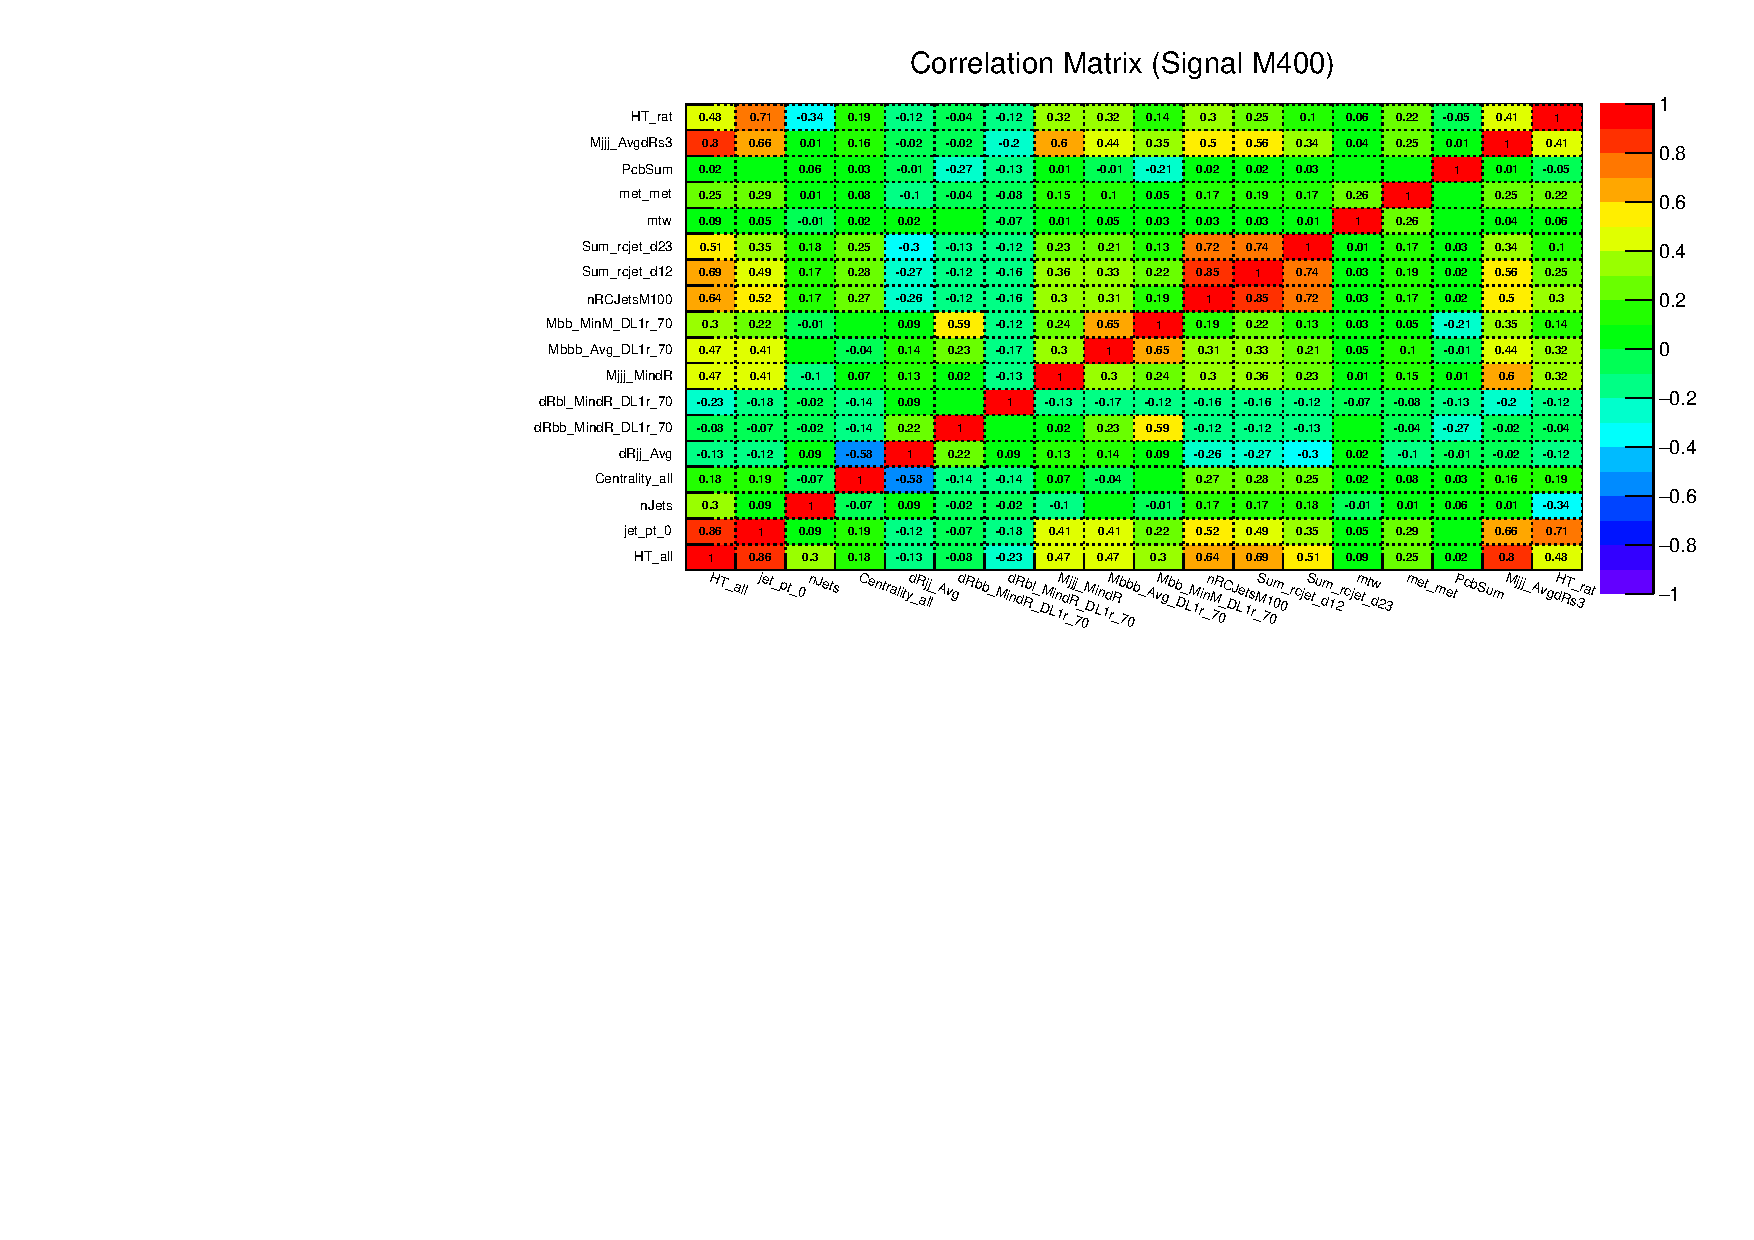
\includegraphics[width=0.55\textwidth]{inputVar_correlation/1L_correlation_m400.pdf}
    \newline
        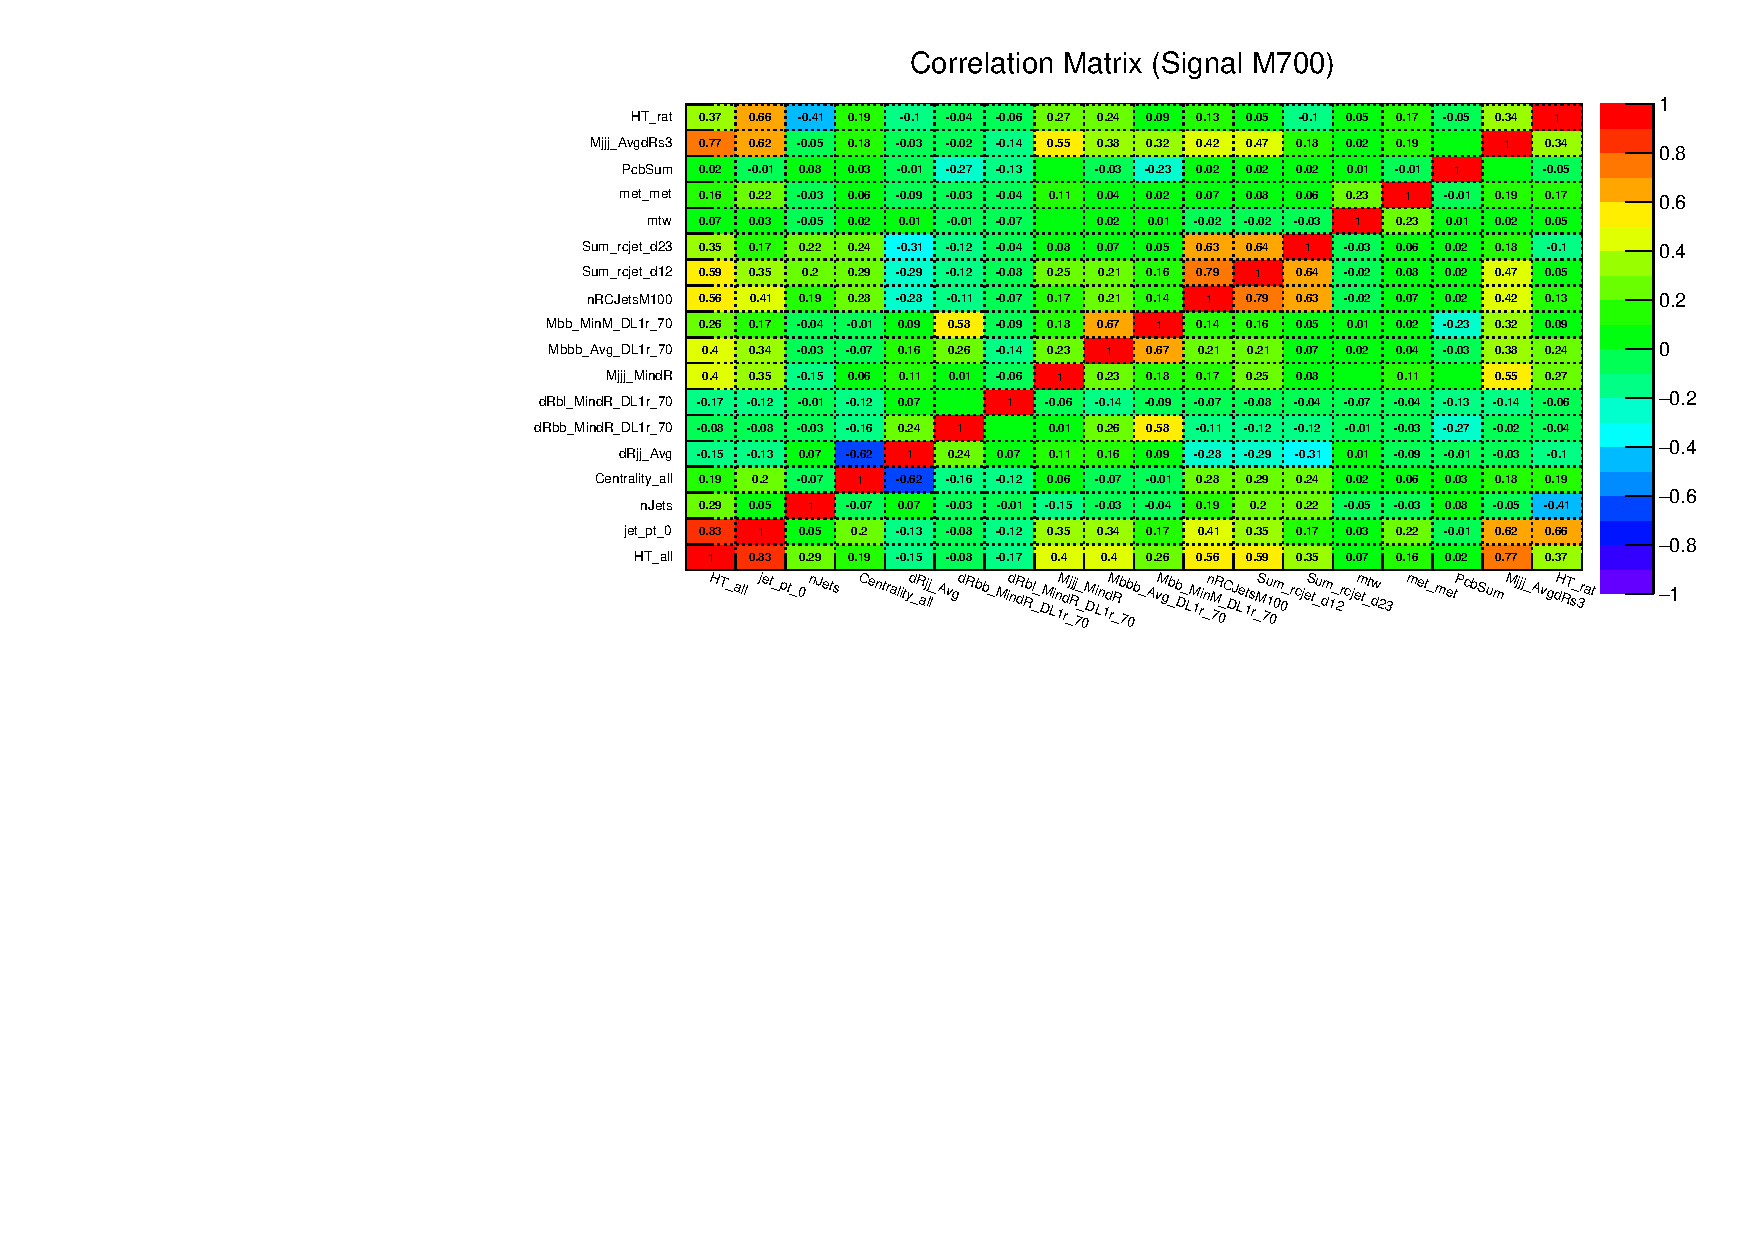
\includegraphics[width=0.55\textwidth]{inputVar_correlation/1L_correlation_m700.pdf}
    \newline    
        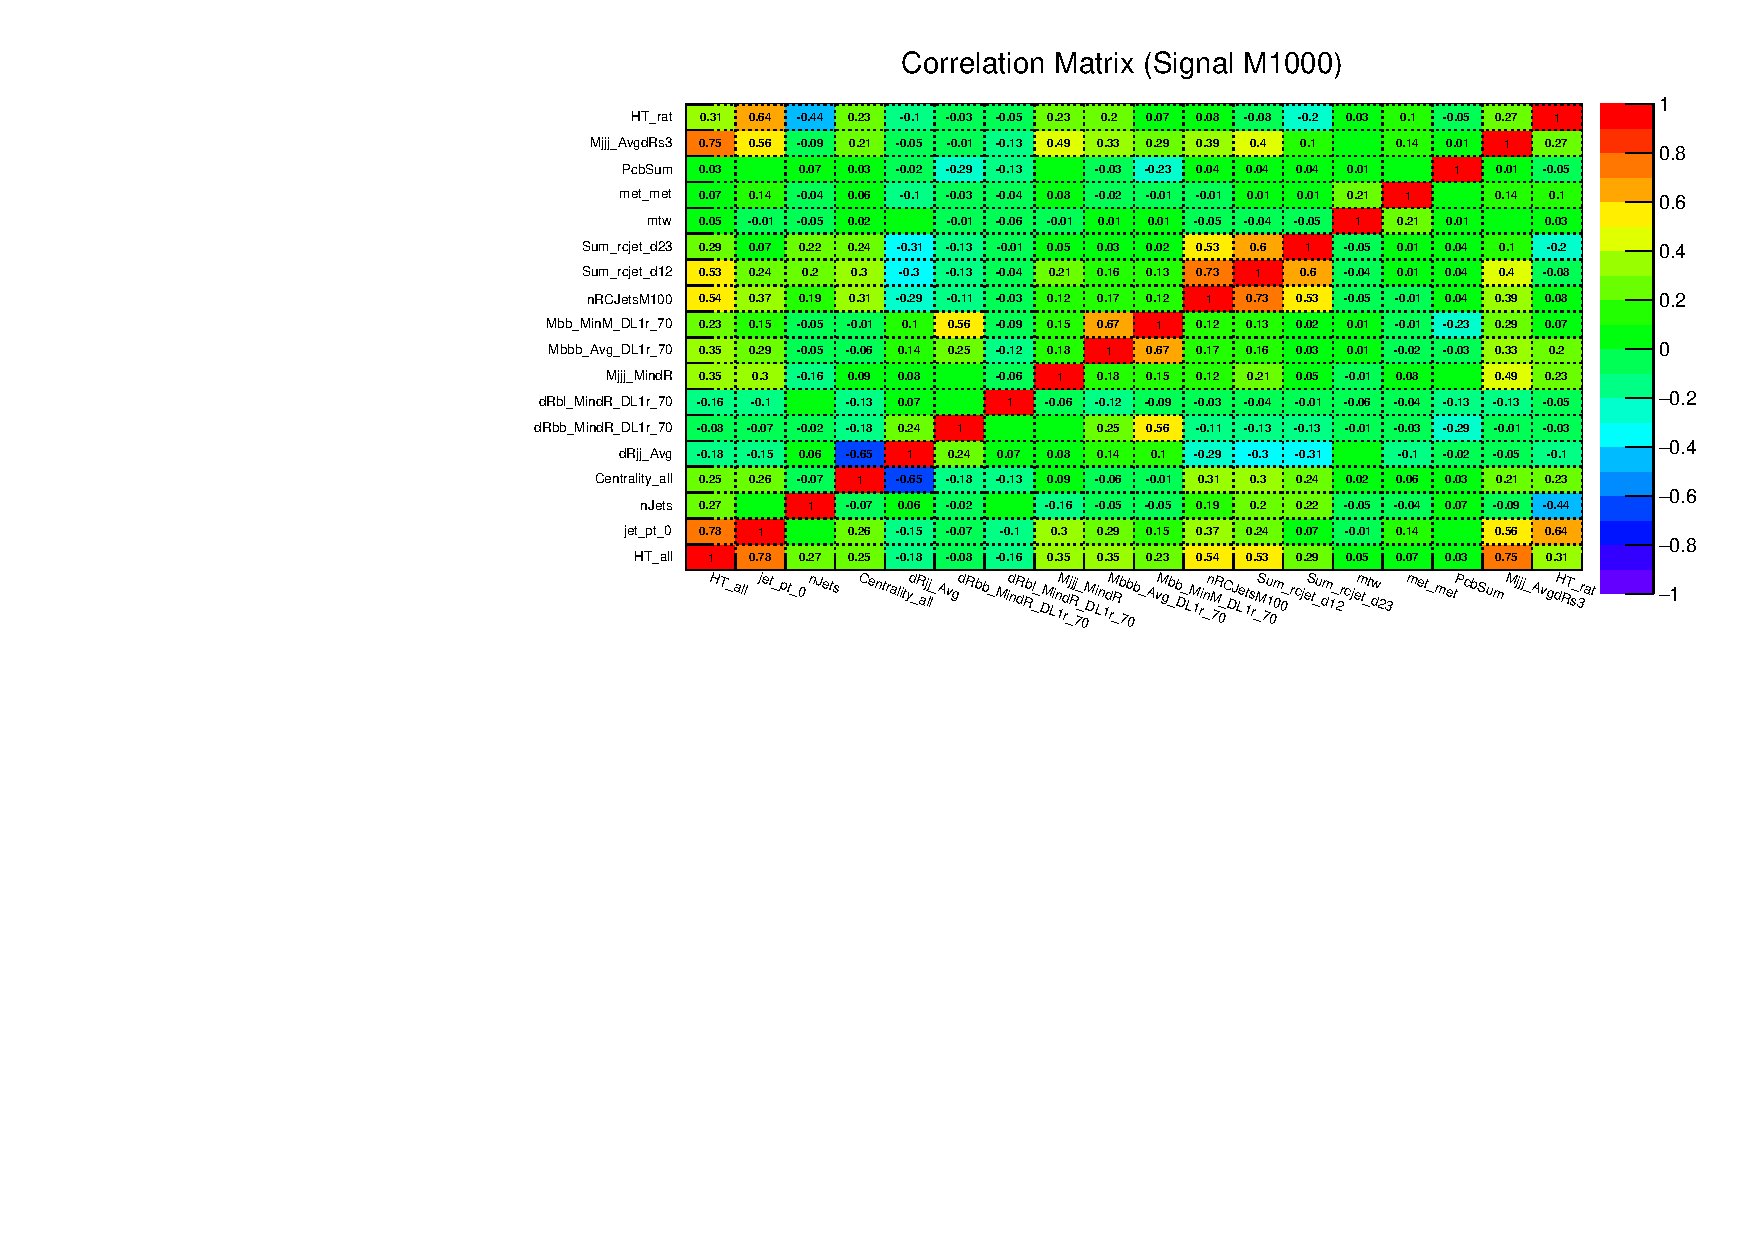
\includegraphics[width=0.55\textwidth]{inputVar_correlation/1L_correlation_m1000.pdf}
    \newline   
    \caption{\label{fig:1L_inputVarCorrelation}The correlation plots of all the input variables in $t\bar{t}$+jets background, and $t\bar{t}H(\rightarrow t\bar{t})$ with BSM Higgs boson mass of 400 GeV, 700 GeV and 1000 GeV in the region of 1L$\geq 9j \geq 3b$. The empty bins correspond to no correlation between variables.}
\end{figure}
%%%%%%%%%

The above input variables have different separation power in the BDT.
The input variables importance indicates the significant of the variables in the BDT.
A simple way to define the feature importance could be an iterative method which is dropping each feature and calculating the Area Under the ROC Curve (AUC) until all features are processed.
It is more convenient to look at the importance in terms of the percentage change:

%%%%Equation: Importance Definition%%%%
\begin{equation}
\mathrm{Imp}[i]\mathrm{=\frac{{AUC}_{ref}-{AUC}_{i}}{\sum_{i}\mid {AUC}_{ref}-{AUC}_{i} \mid}}~,
\end{equation}
%%%%%%%%%%%%%%%%%%%%%%%%%%%%%%%%%%%%%%%
where $\mathrm{Imp}[i]$ is the importance of input variable with index $i$, $\mathrm{AUC_{ref}}$ is the AUC value of the BDT with all input variables and $\mathrm{AUC_{i}}$ is the AUC value of the BDT trained without input variable $i$.
These AUC values are calculated from the BDT with the nominal hyper-parameters which are discussed in the next sub-section.
Figure~\ref{fig:1L_Importance} shows the importance rank of input variables in different signal mass points BDT are not identical.

%%%%Fig: Importance%%%%
\begin{figure}[!htp]\centering
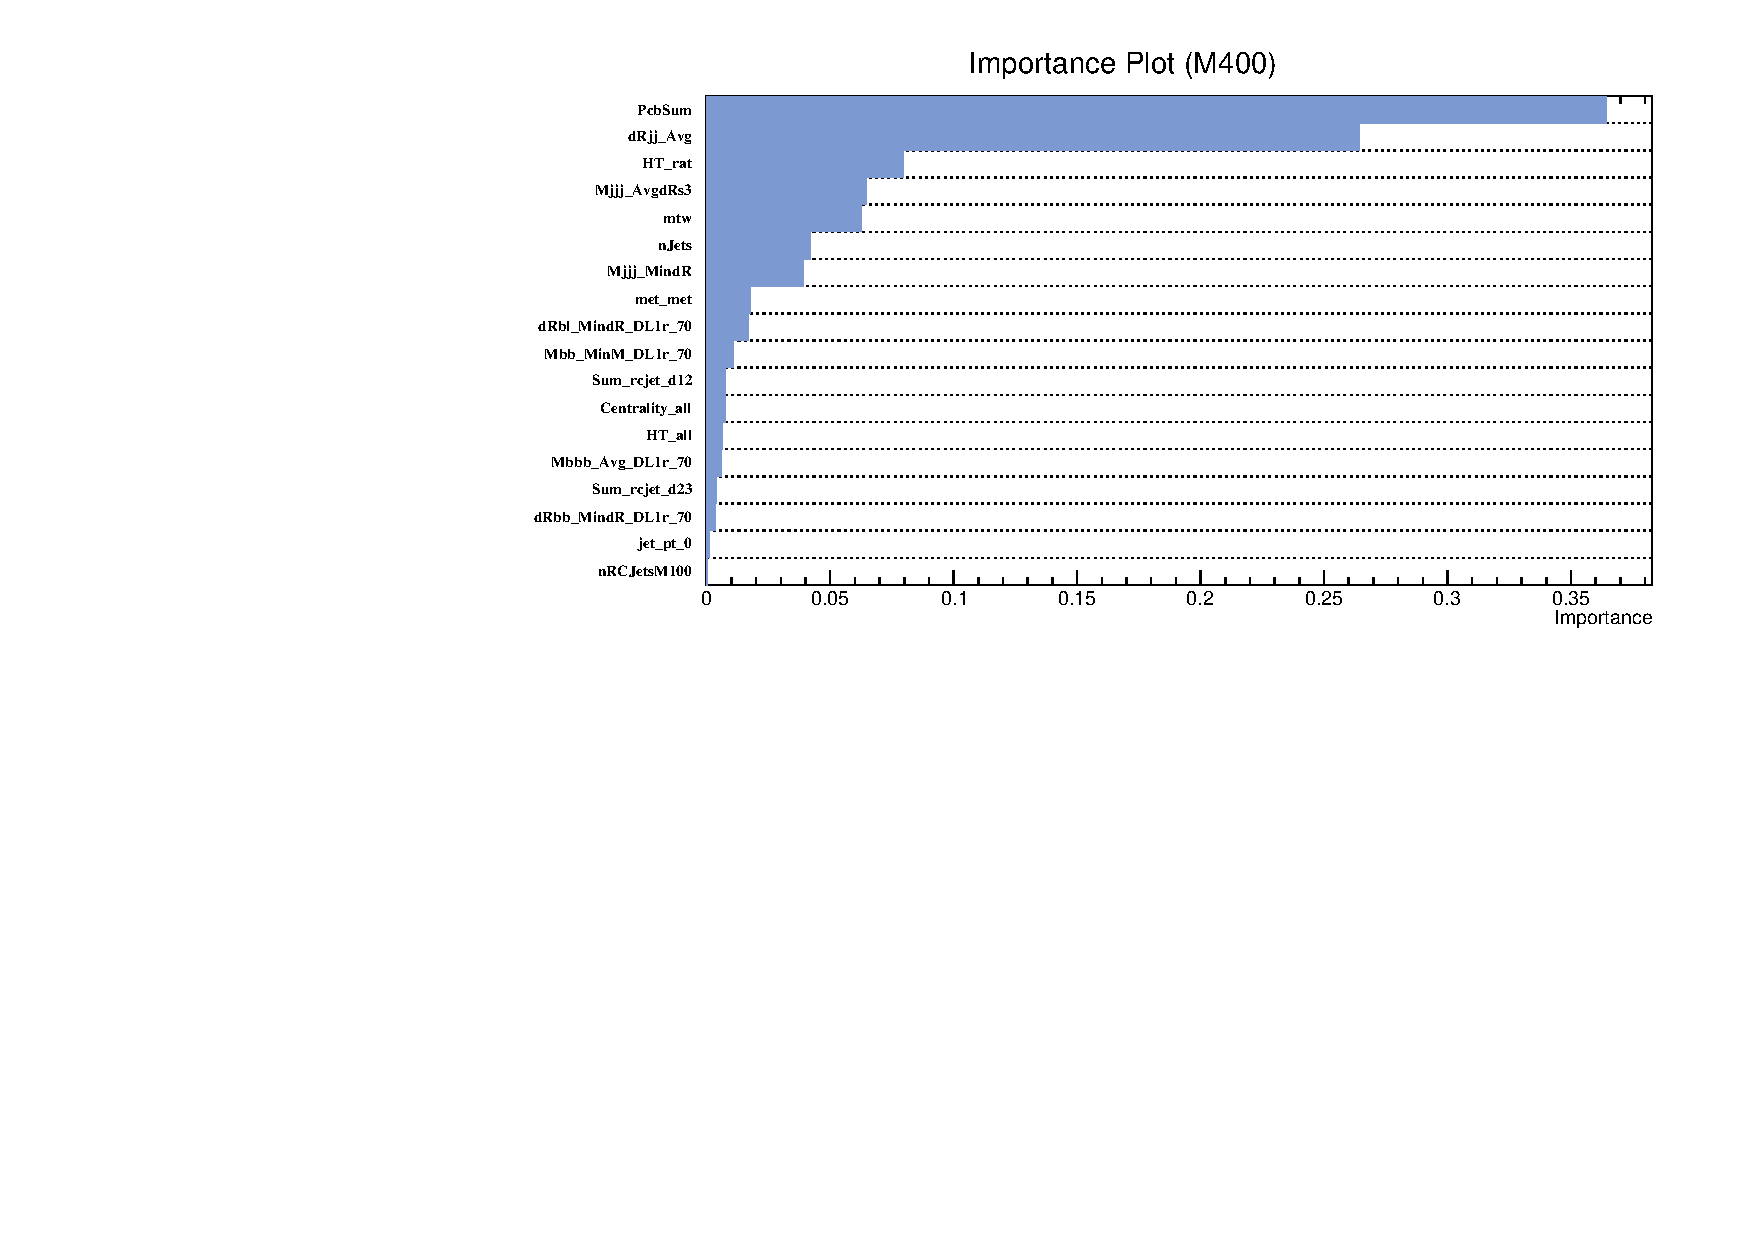
\includegraphics[width=0.75\textwidth]{importance/1L_varImp_M400.pdf}
\\
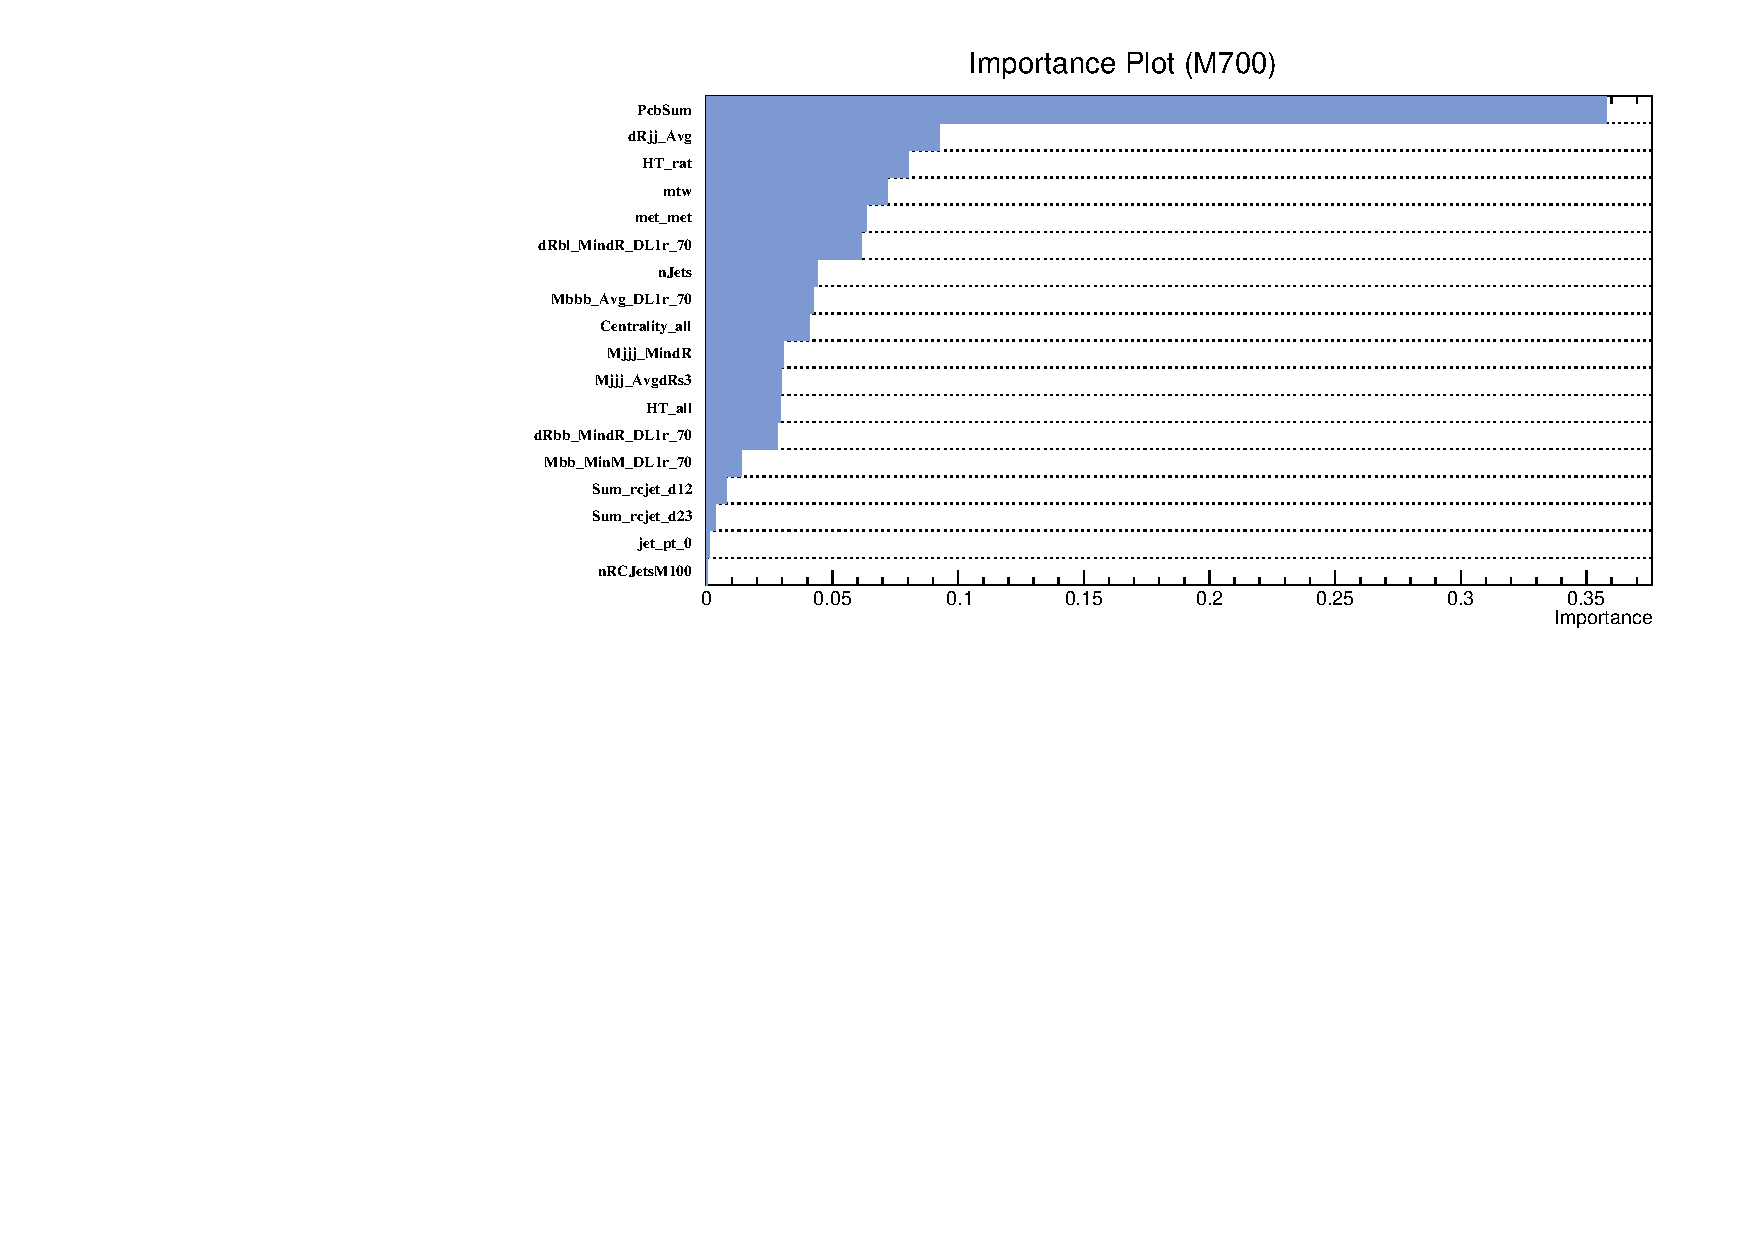
\includegraphics[width=0.75\textwidth]{importance/1L_varImp_M700.pdf}
\\
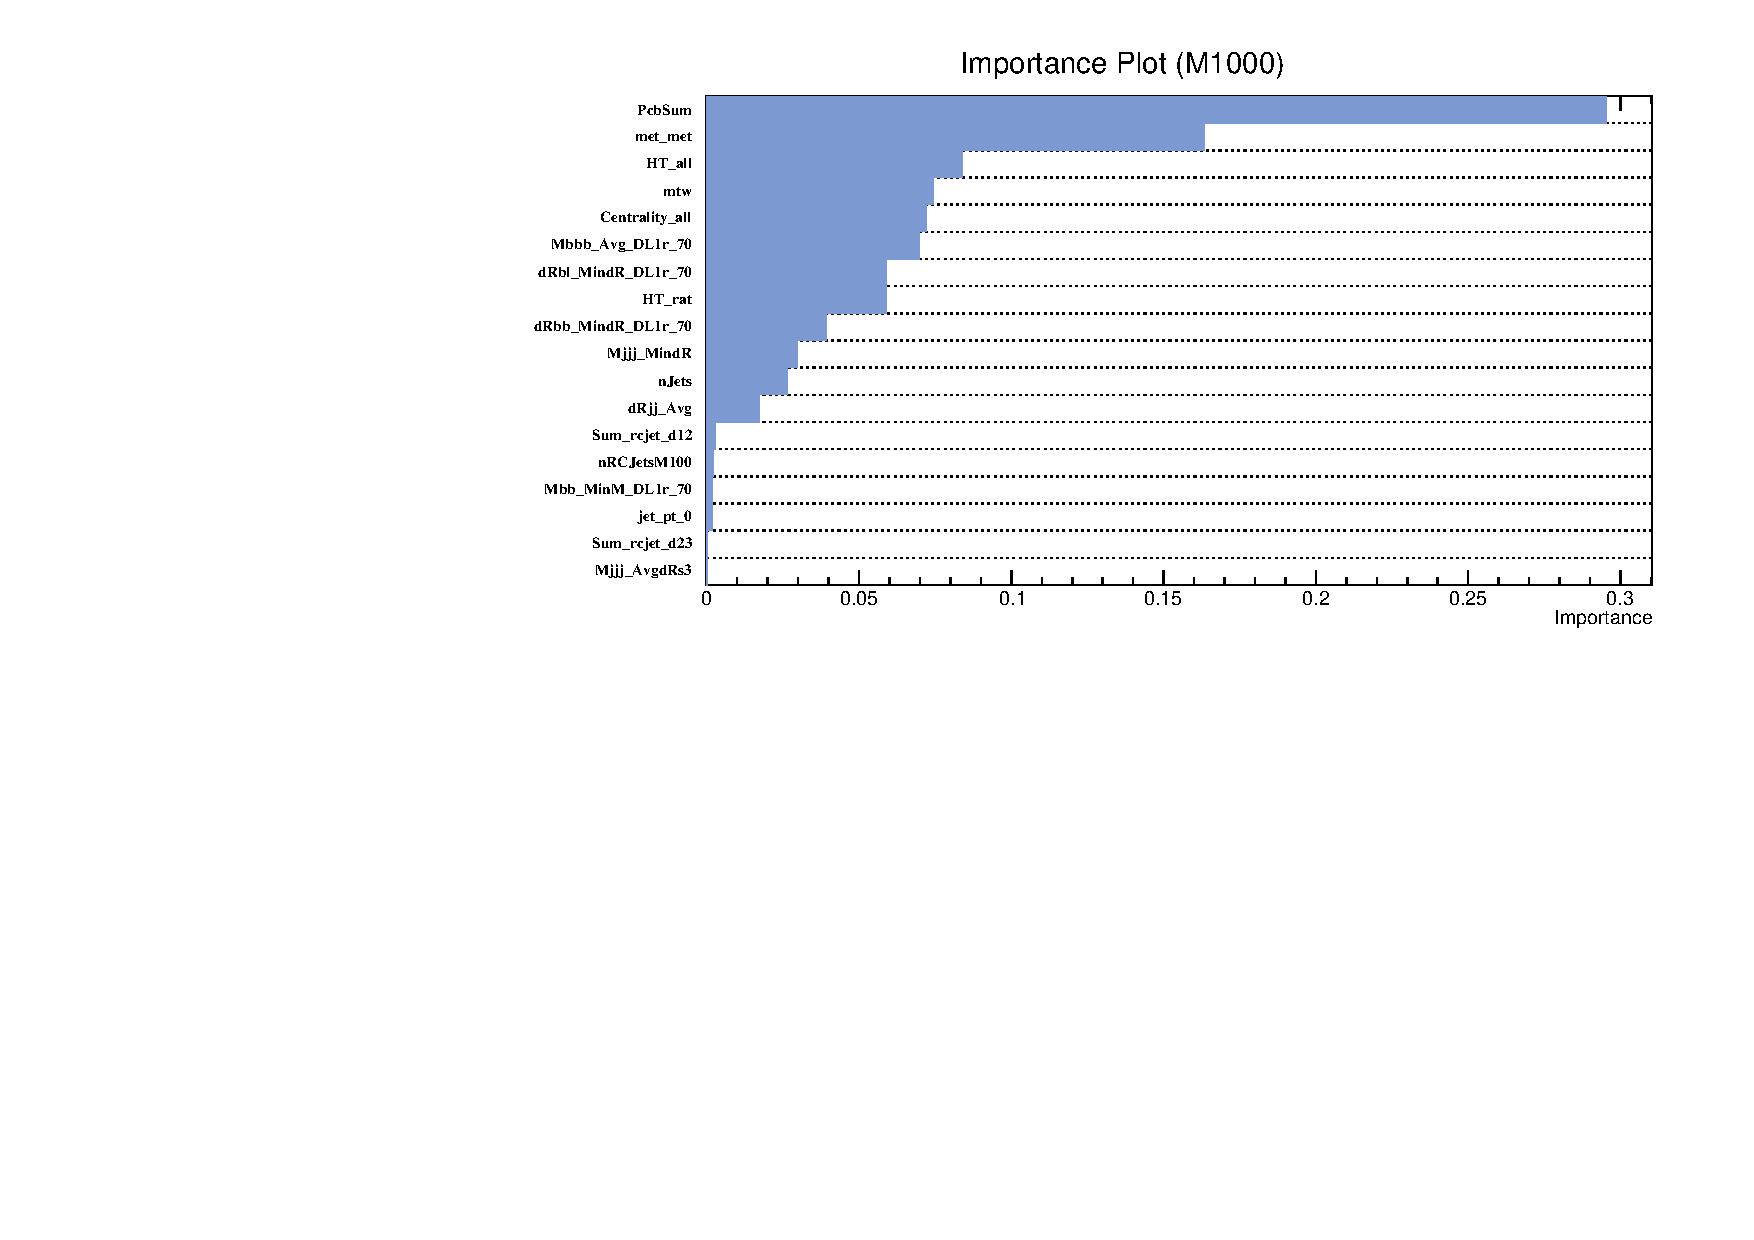
\includegraphics[width=0.75\textwidth]{importance/1L_varImp_M1000.pdf}
\caption{\label{fig:1L_Importance} The importance ranking of input variables in the BDT with BSM Higgs boson mass of (a) $400~GeV$, (b) $700~GeV$ and (c) $1000~GeV$ in $t\bar{t}H(\rightarrow t\bar{t})$ in 1L channel.}

\end{figure}

\begin{figure}[!htp]\centering
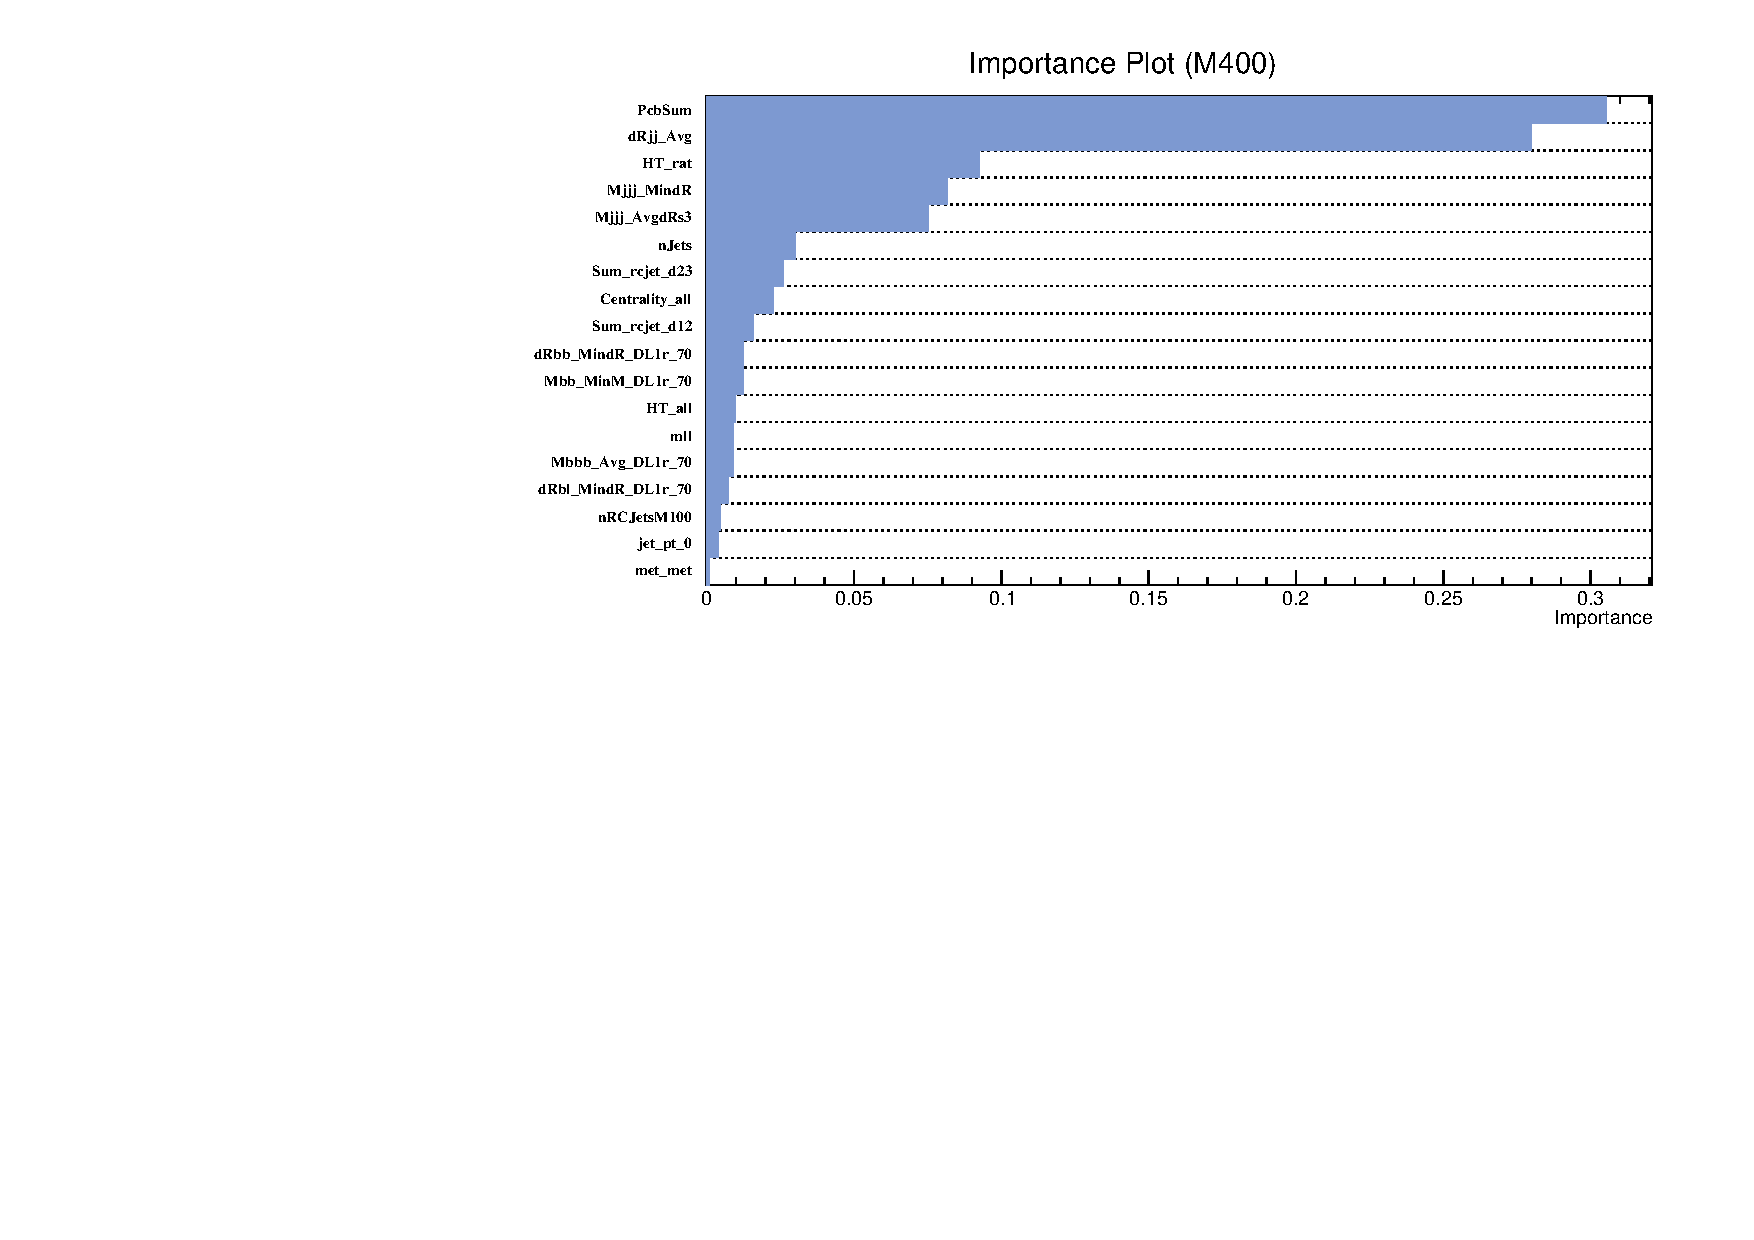
\includegraphics[width=0.75\textwidth]{importance/2LOS_varImp_M400.pdf}
\\
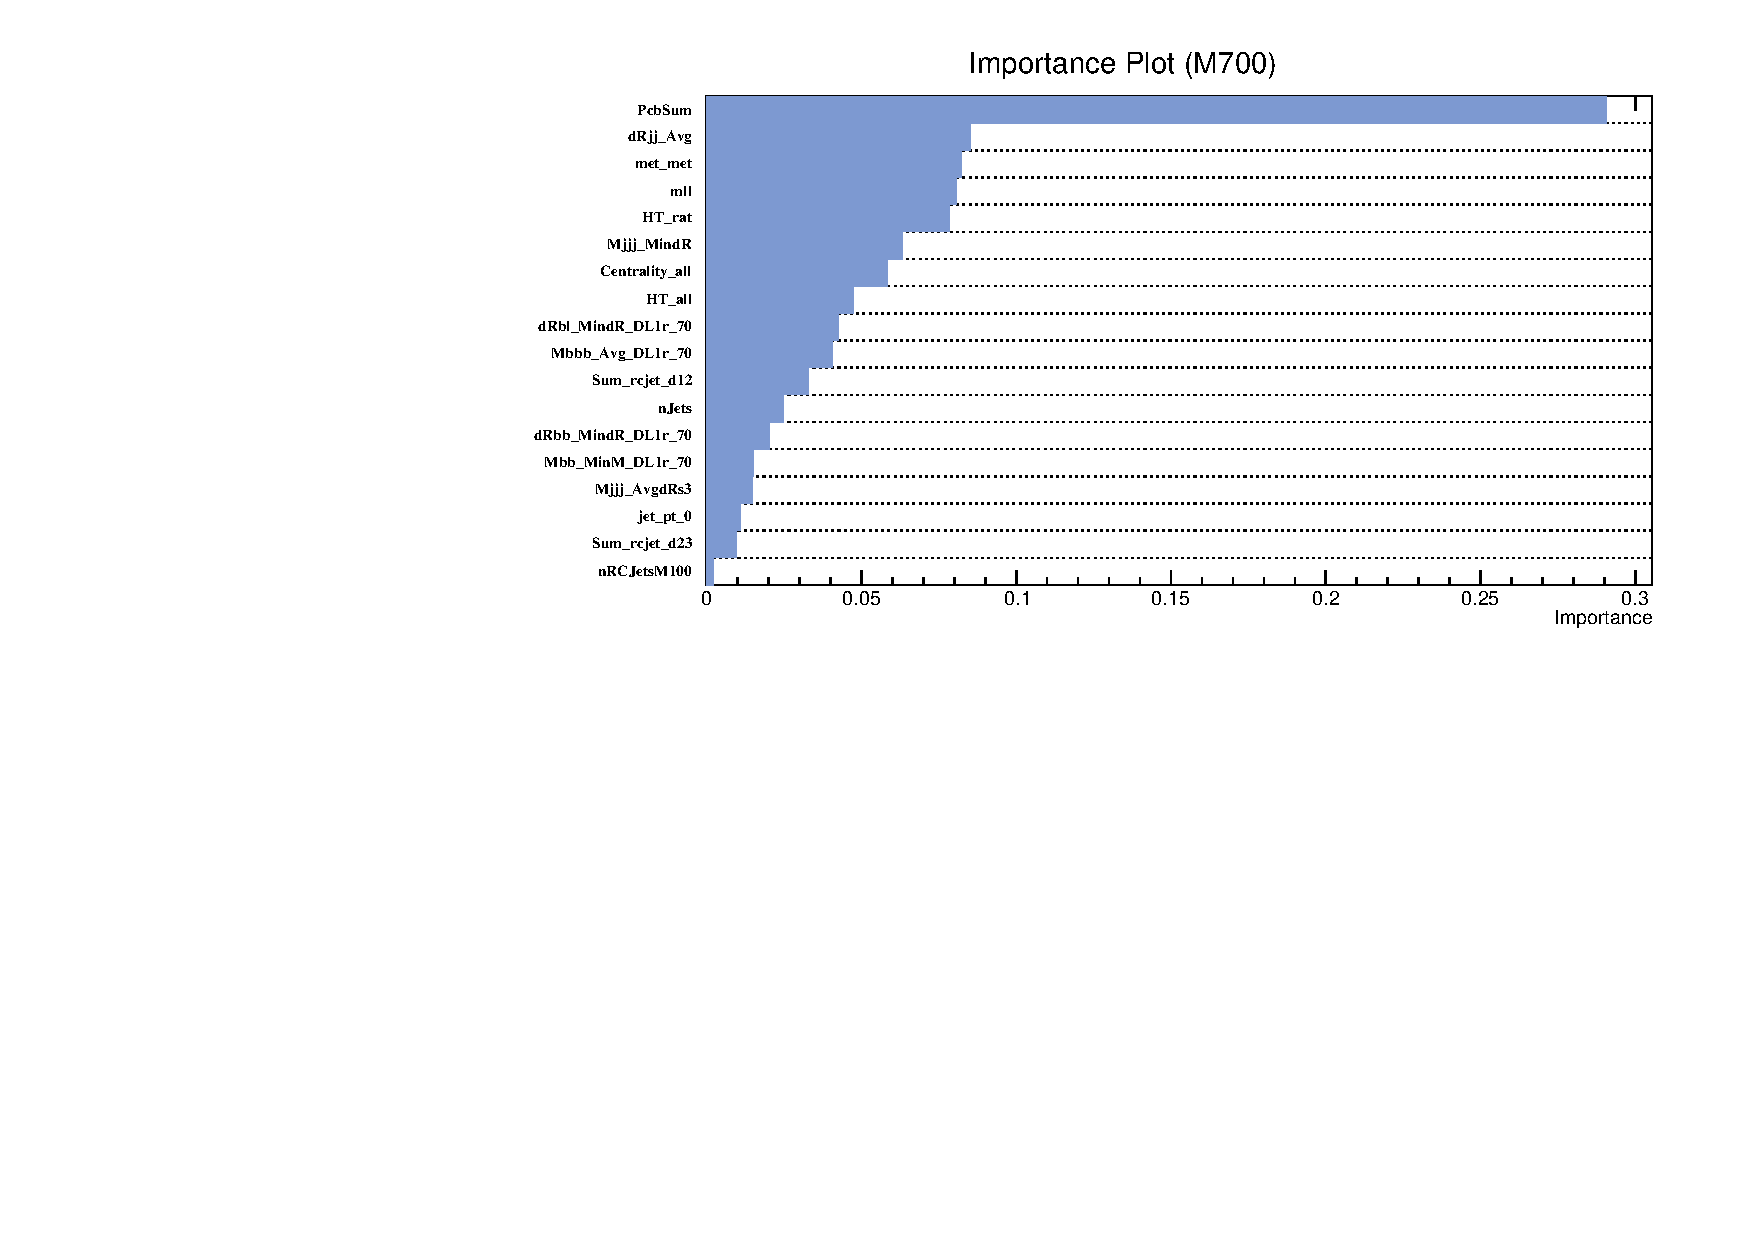
\includegraphics[width=0.75\textwidth]{importance/2LOS_varImp_M700.pdf}
\\
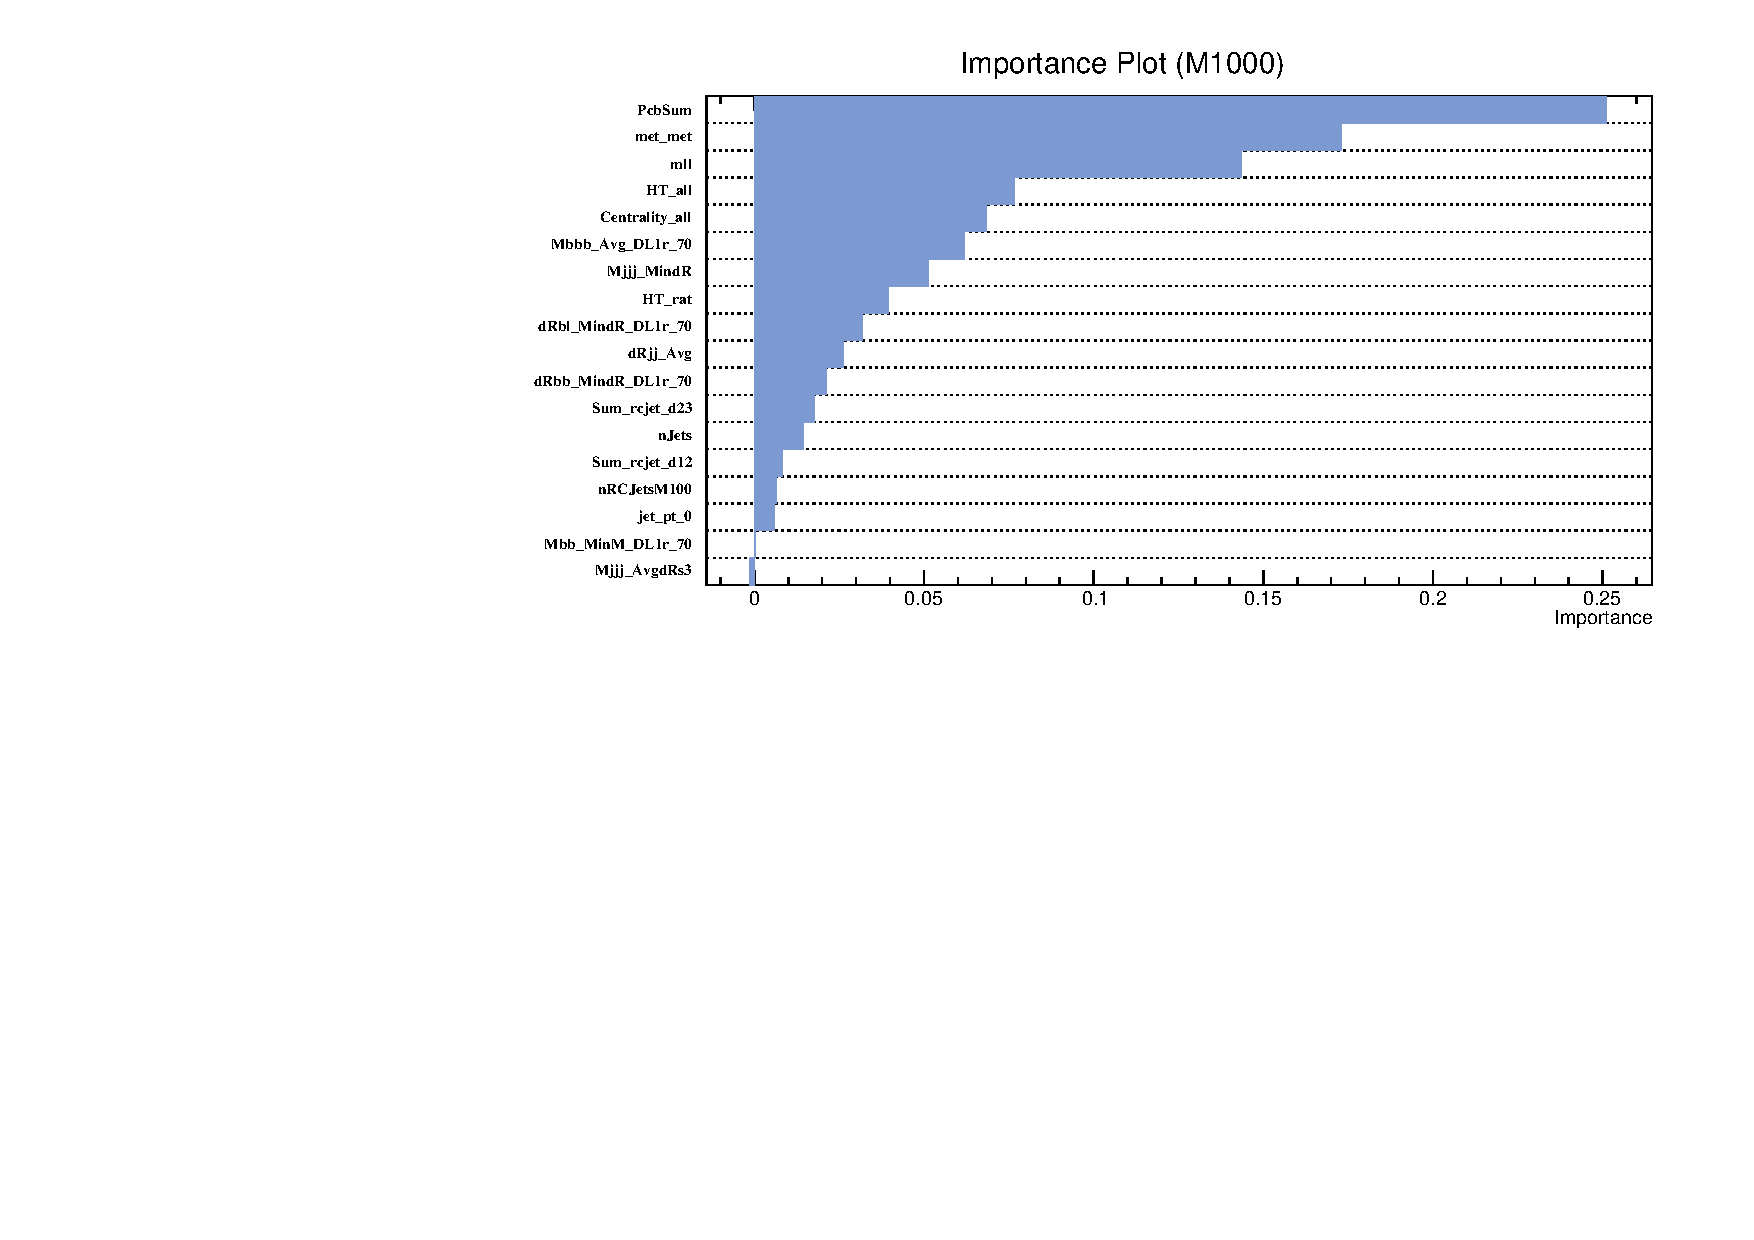
\includegraphics[width=0.75\textwidth]{importance/2LOS_varImp_M1000.pdf}
\caption{\label{fig:2LOS_Importance} The importance ranking of input variables in the BDT with BSM Higgs boson mass of (a) $400~GeV$, (b) $700~GeV$ and (c) $1000~GeV$ in $t\bar{t}H(\rightarrow t\bar{t})$ in 2LOS channel.}

\end{figure}
%%%%%%%%%%%%%%%%%%%%%%%%%%%%

%%%%Table: BDT Variable Rank %%%%
\begin{table}[!htp]
    \centering
\resizebox*{\textwidth}{!}{
    \begin{tabular}{|c||c|c|c||c|c|c||c|c|c|}
        \hline
        &\multicolumn{3}{c|}{M400} & \multicolumn{3}{c|}{M700} & \multicolumn{3}{c|}{M1000}\\
        \hline \hline
        Variable & AUC reduction & Separation & TMVA Importance & AUC reduction & Separation & TMVA Importance & AUC reduction & Separation & TMVA Importance \\
        \hline
        $H_{T}$ & 13 & 9 & 10 & 12 & 1 & 12 & 3 & 1 & 1 \\
        $\sum_{i} {p_{T}}_{i}/ \sum_{i} E_{i}$ & 12 & 3 & 9 & 9 & 9 & 5 & 5 & 10 & 3 \\
        $N_{jets}$ & 6 & 4 & 14 & 7 & 6 & 15 & 11 & 9 & 16 \\
        ${p_{T}}_{0}$ & 17 & 15 & 13 & 17 & 10 & 16 & 16 & 5 & 14 \\
        $\Delta R^{avg}_{jj}$ & 2 & 2 & 1 & 2 & 12 & 2 & 12 & 14 & 11 \\
        $M^{min. \Delta R}_{jjj}$ & 7 & 11 & 5 & 10 & 11 & 11 & 10 & 8 & 10 \\
        $M^{\Delta R<3}_{jjj}$ & 4 & 5 & 4 & 11 & 2 & 9 & 18 & 2 & 12 \\
        $\sum^{3}_{i=0}{p_{T}}_{i} / \sum_{i\geq 4} {p_{T}}_{i}$ & 3 & 6 & 2 & 3 & 16 & 1 & 8 & 17 & 2 \\
        $\Delta R^{min}_{bl}$ & 9 & 18 & 8 & 6 & 18 & 4 & 7 & 16 & 5 \\
        $\Delta R^{min}_{bb}$ & 16 & 14 & 6 & 13 & 17 & 10 & 9 & 18 & 8 \\
        $M^{avg}_{bbb}$ & 14 & 12 & 12 & 8 & 8 & 6 & 6 & 6 & 7 \\
        $M^{min}_{bb}$ & 10 & 16 & 11 & 14 & 13 & 13 & 15 & 12 & 17 \\
        $\sum^{i<4}_{i=0} {pcb}_{i}$ & 1 & 1 & 3 & 1 & 5 & 3 & 1 & 11 & 6 \\
        $N_{RC100}$ & 18 & 10 & 18 & 18 & 4 & 18 & 14 & 4 & 18 \\
        $\sum d_{12}$ & 11 & 7 & 16 & 15 & 3 & 14 & 13 & 3 & 13 \\
        $\sum d_{23}$ & 15 & 8 & 17 & 16 & 7 & 17 & 17 & 7 & 15 \\
        $E^{miss}_{T}$ & 8 & 17 & 15 & 5 & 14 & 8 & 2 & 13 & 4 \\
        $m_{T}(\ell,E^{miss}_{T})$ & 5 & 13 & 7 & 4 & 15 & 7 & 4 & 15 & 9 \\
        \hline
    \end{tabular}
}
\caption{BDT input variables ranking based on different method in 1L channel. \label{tab:variableRank_1L}}
\end{table}

%%%%%%%%%%%%%%%%%%%%%%%%%%%%%%%%%

%%%%Next Sub-section%%%%
\subsubsection{Hyper-parameters}

The BDT has several hyper-parameters which are relevant to this study:

\begin{itemize}
\item Boosting algorithm
\item Number of trees (Number of boosting iteration) (NTrees)
\item Learning rate to control the sample overfitting ($\eta$)
\item Bagged sample fraction which creates a sub-sample with certain fraction in training sample including replacement and are used in each boosting iteration  
\item Separation method of node splitting during tree training
\item Number of gird points in input variable range used to represent the optimal cut in node splitting (nCuts)
\item Maximum tree depth allowed (MaxDepth)
\end{itemize}

The hyper-parameters setup are optimized by scanning the average AUC-value among all the signal mass points in the testing BDT and the average AUC difference between training and testing BDT with different hyper-parameters combination.
A high AUC-value implies a high separation between signal and background while a low AUC difference indicates no overtraining.

In the optimization study, the boosting algorithm is fixed to Gradient Boost with bagging fraction 60\%.
The separation method in a node splitting is chosen to be Gini Index.
The remaining parameters are scanned in 300 combinations with different NTrees, $\eta$, nCuts and MaxDepth, as shown in Table~\ref{tab:hyperParameterScan}.
Figure~\ref{fig:1LHyperParaT600} and Figure~\ref{fig:1LHyperParaT1000} show the results from the hyper-parameters scan at NTrees$=600$ and $1000$ respectively in 1L$\geq 9j\geq 3b$ region.
Since no big improvement on the sensitivity is found after the hyper-parameters optimization, the BDT hyper-parameters in this analysis are chosen to be the same as those in the SM4t studies:

\begin{itemize}
\item Number of trees: 600
\item Boosting: Gradient with bagging (sample fraction of 0.6)
\item Learning-rate: 0.05
\item Loss function: GiniIndex
\item Number of scanned cuts: 30
\item Maximum tree depth: 2
\end{itemize}

%%%%Table: Hyperparameter Scan%%%%
\begin{table}[!htp]
    \centering
    \begin{tabular}{|c|c|c|c|}
        \hline
        NTrees & $\eta$ & nCuts & MaxDepth \\
        \hline
        200 & 0.01 & 25 & 2\\
        400 & 0.02 & 30 & 3\\
        600 & 0.05 & 35 & 4\\
        800 & 0.10 &    & \\
        1000 & 0.20 &   &  \\
        \hline
    \end{tabular}
\caption{Different hyper-parameters scanning points. \label{tab:hyperParameterScan}}
\end{table}
%%%%%%%%%%%%%%%%%%%%%%%%%%%%%%%%%

%%%%Figure : Hyperparameter Scan T600 %%%%
\begin{figure}[!htp]
    \centering
        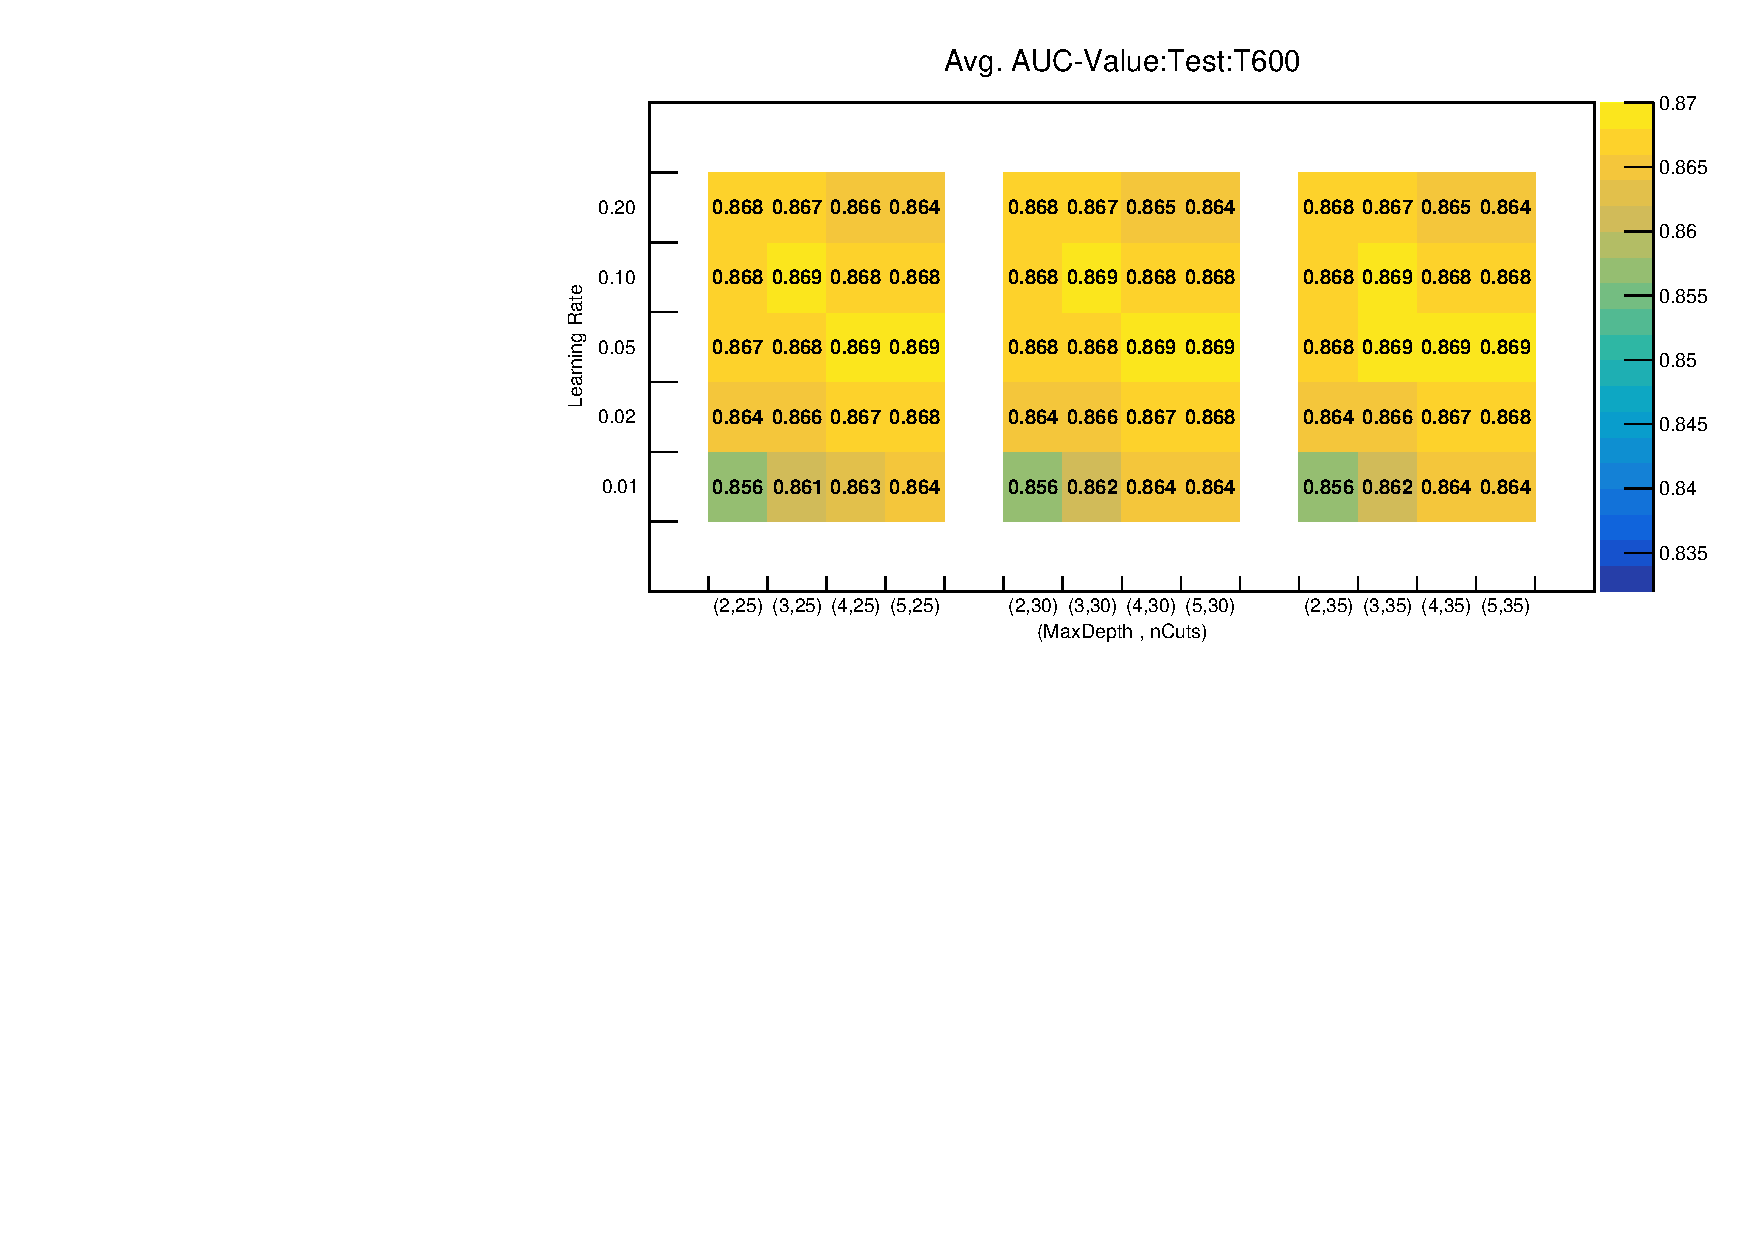
\includegraphics[width=0.55\textwidth]{hyperParameter/T600_test_1L.pdf}
        \subcaption{Average AUC Value of Testing with NTrees 600}
        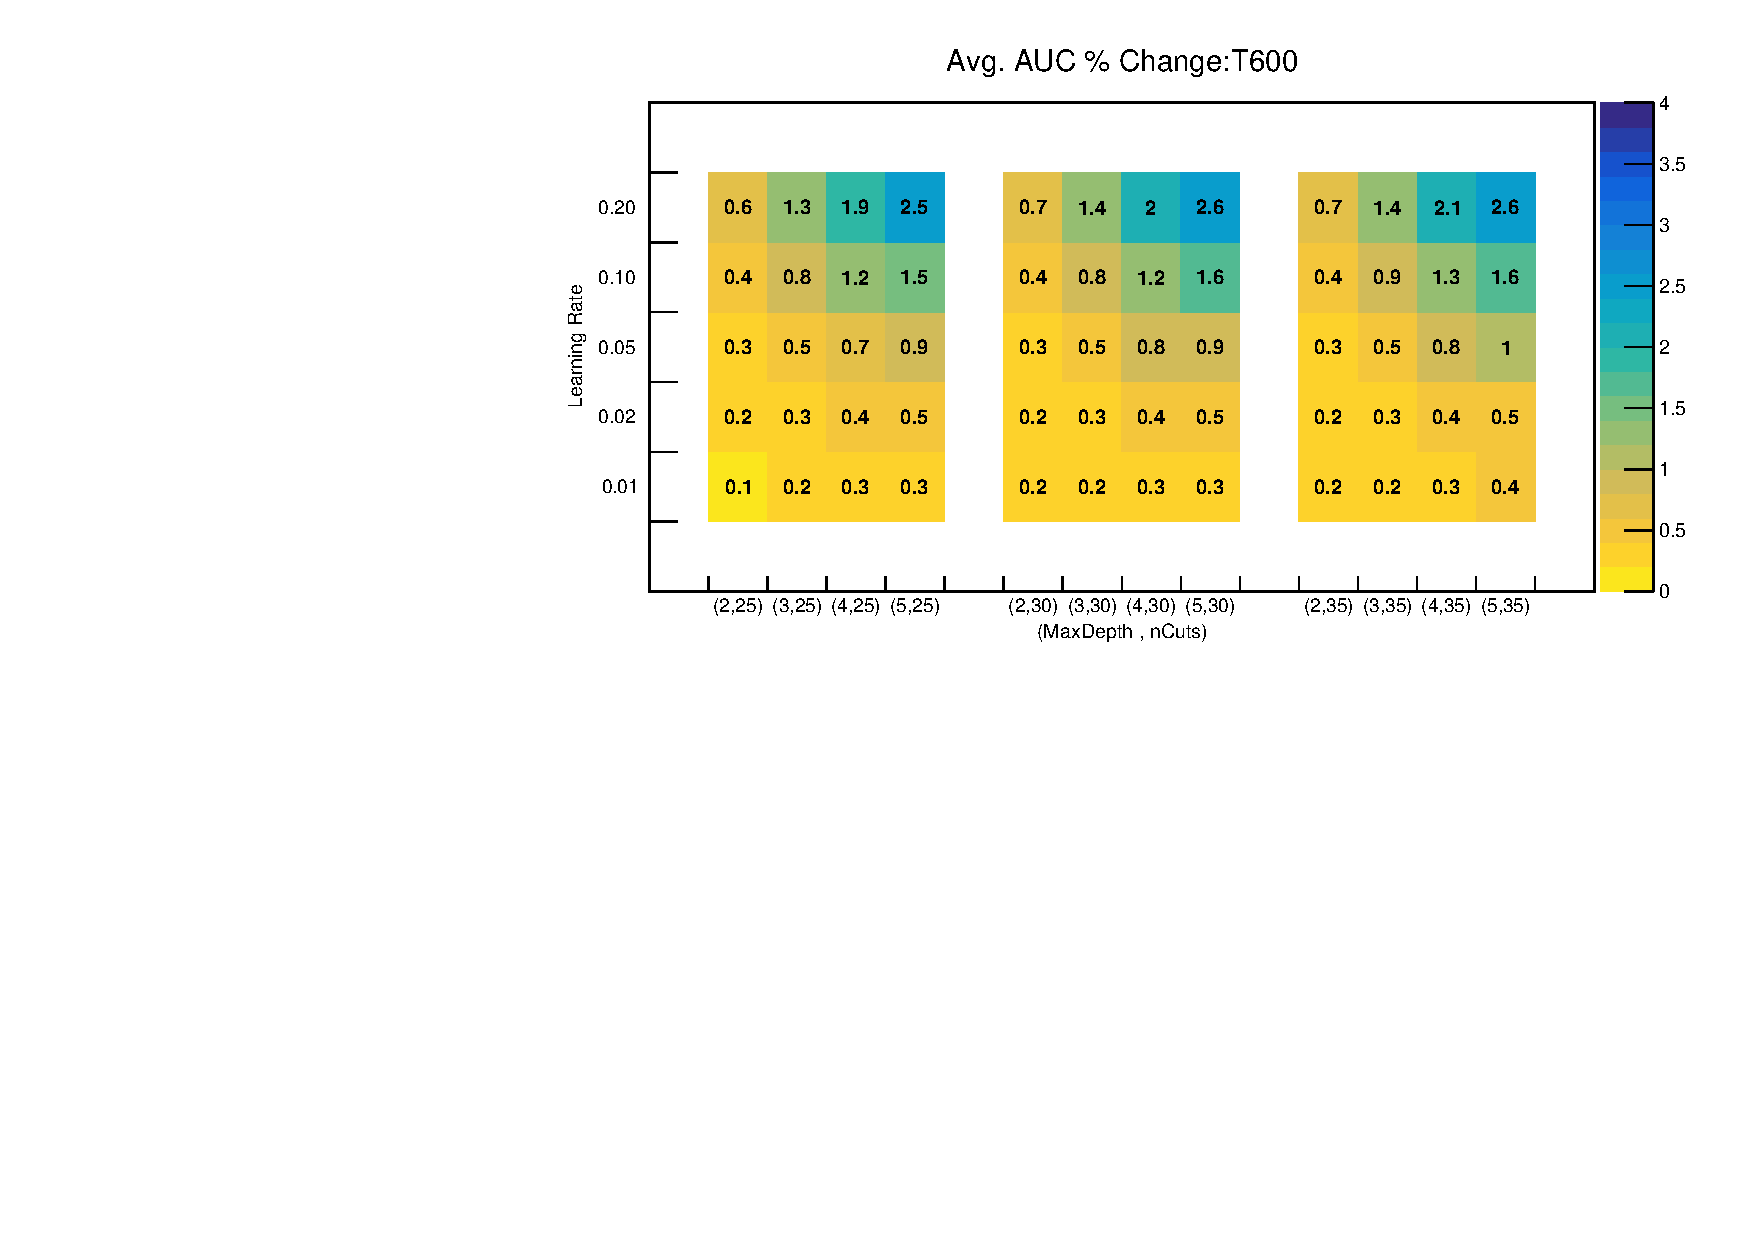
\includegraphics[width=0.55\textwidth]{hyperParameter/T600_val_1L.pdf}
        \subcaption{Average AUC \% Change with NTrees 600}
    \caption{\label{fig:1LHyperParaT600}Hyper-parameter scan at learning-rate, maximum tree depth and the number of cuts in the input variables by fixing the number of trees into 600. Figure (a) gives the average AUC-value in the test BDT with different hyper-parameter setup while figure (b) gives the AUC \% difference between train and test BDT, which is defined as $\mathrm{(AUC^{avg}_{train}-AUC^{avg}_{test})/AUC^{avg}_{train}}\times 100$. The scan is performed in 1L$\geq 9j \geq 3b$ region}
\end{figure}    
%%%%%%%%%%%%%%%%%%%%%%%%%%%%%%%%%%%%%%%%%    

%%%%Figure : Hyperparameter Scan T600 %%%%
\begin{figure}[!htp]
    \centering
%    \subfloat[Average AUC Value of Testing with NTrees 1000]{
        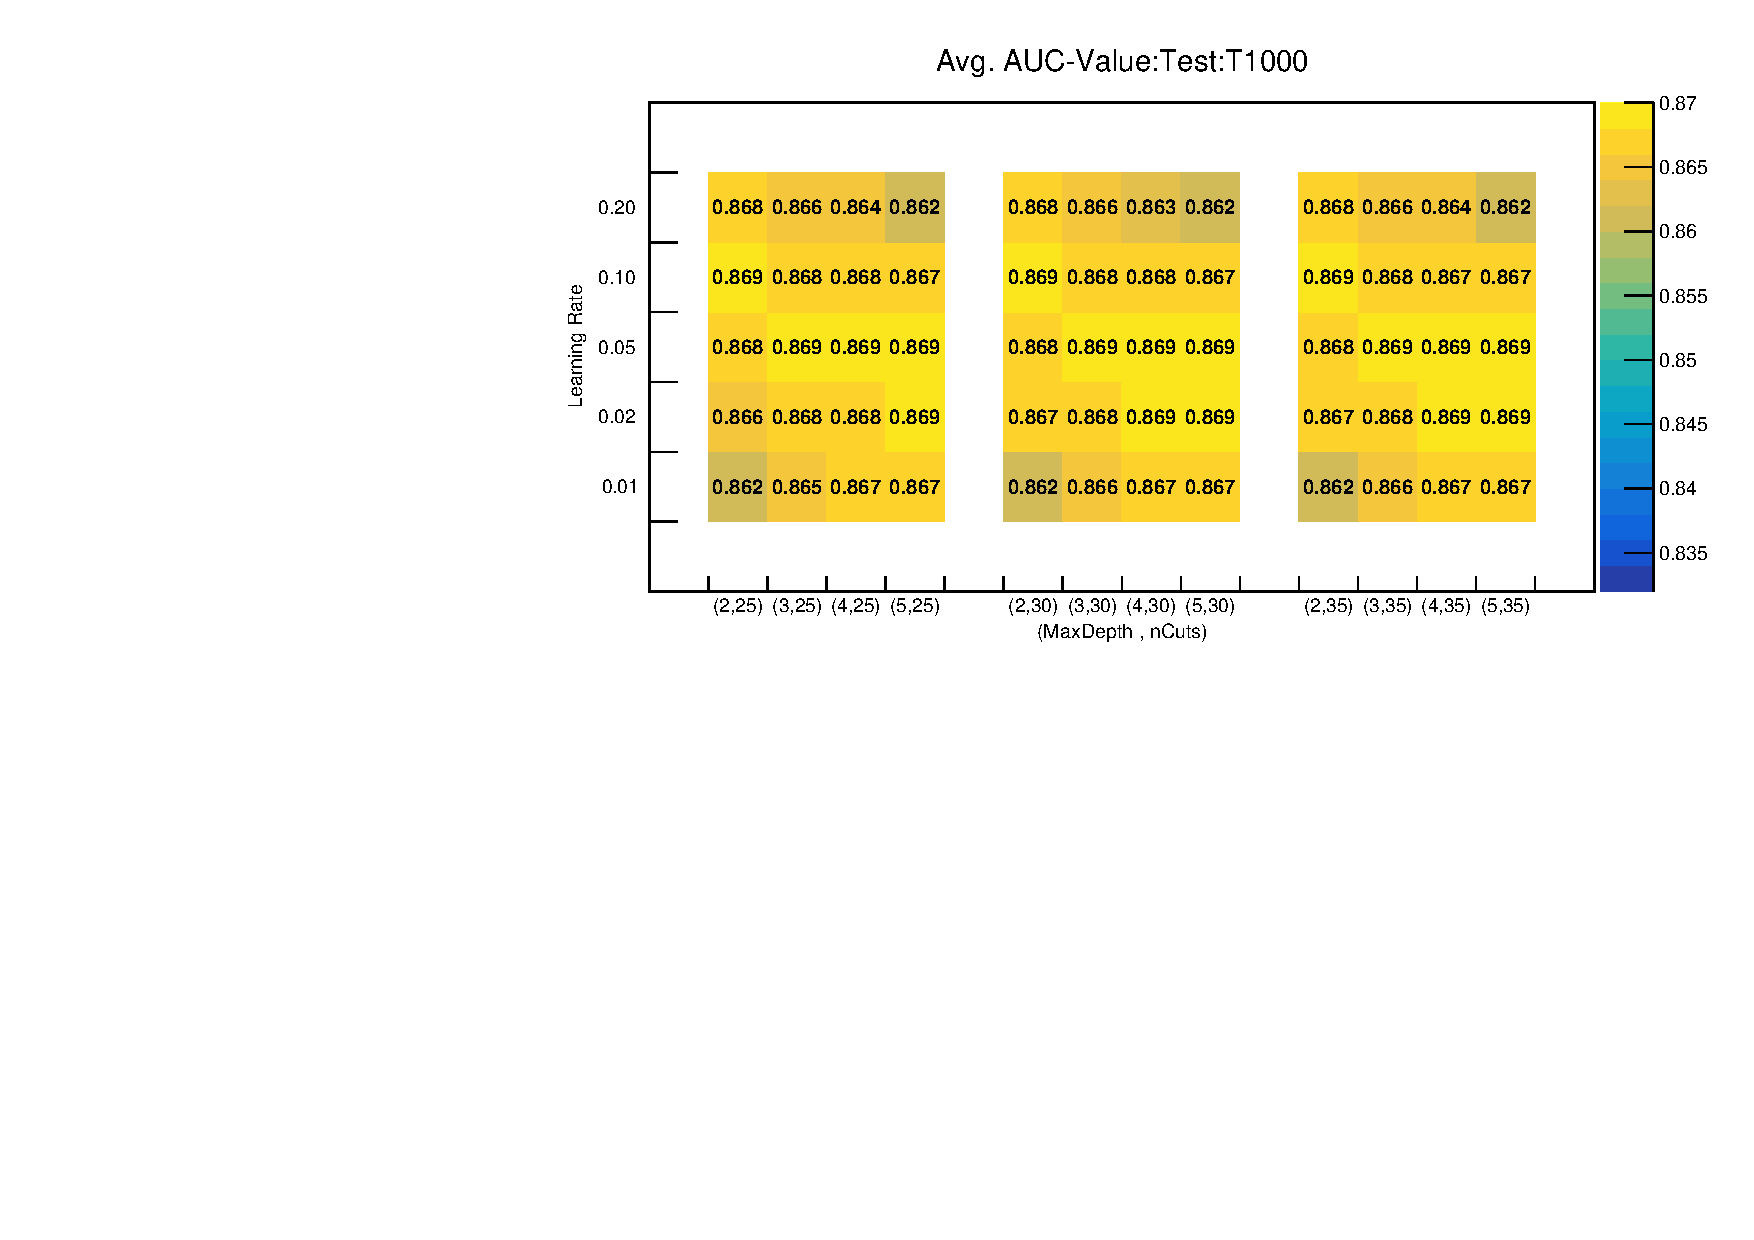
\includegraphics[width=0.55\textwidth]{hyperParameter/T1000_test_1L.pdf}
%    }
%    \subfloat[Average AUC \% Change with NTrees 1000]{
        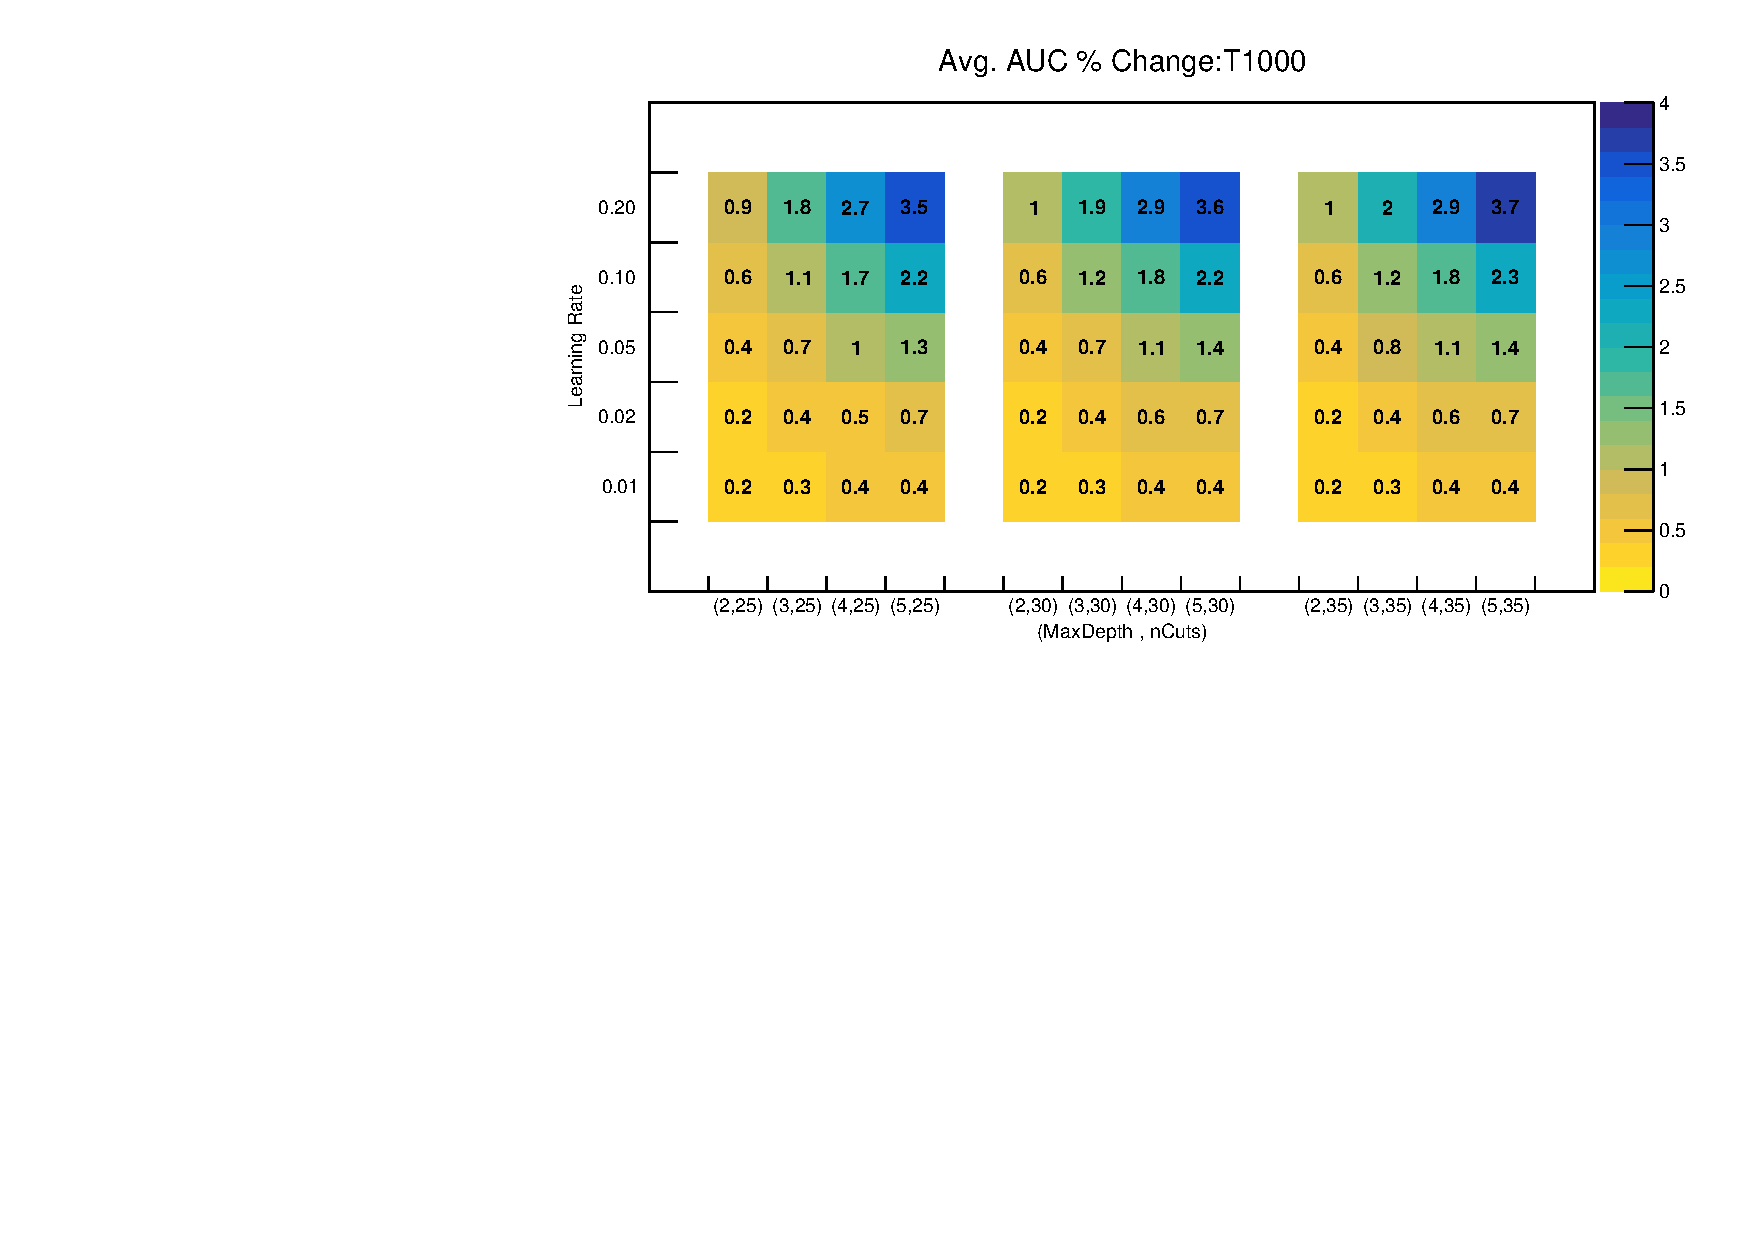
\includegraphics[width=0.55\textwidth]{hyperParameter/T1000_val_1L.pdf}
%    }
    \caption{\label{fig:1LHyperParaT1000}Hyper-parameter scan at learning-rate, maximum tree depth and the number of cuts in the input variables by fixing the number of trees into 1000. Figure (a) gives the average AUC-value in the test BDT with different hyper-parameter setup while figure (b) gives the AUC \% difference between train and test BDT, which is defined as $\mathrm{(AUC^{avg}_{train}-AUC^{avg}_{test})/AUC^{avg}_{train}}\times 100$. The scan is performed in 1L$\geq 9j \geq 3b$ region}
\end{figure}    
%%%%%%%%%%%%%%%%%%%%%%%%%%%%%%%%%%%%%%%%% 

%%%%Next Sub-section%%%%
\subsubsection{Performance of BDT}
The BDT performance is evaluated by the AUC value of the ROC curve and the overtraing check.
Overtraining is checked by comparing the AUC value between the training and the testing BDT in the combination of even and odd samples.
The AUC value increases with the signal mass points used in the BDT training, from $0.81$ for M400 to $0.91$ for M1000 while the deviations of testing BDT AUC value from the training one is within $0.6$ \% for all the signal mass points in the region of 1L$\geq 9j \geq 3b$.
Figure~\ref{fig:1Lge9jge3bBDT} provides the distribution of BDT and ROC of signal mass points M400, M700 and M1000 in 1L$\geq 9j\geq 3b$ region.
A trend of AUC value in the signal mass points is shown in Figure~\ref{fig:AUC_perMP}, that the AUC value increases with the signal mass point because the separation of most of the variables between signal and background increases with the BSM Higgs boson mass.
 
%%%%Fig: 1L BDT and ROC%%%%
\begin{figure}[!htp]\centering
   \begin{subfigure}[t]{0.49\textwidth}
        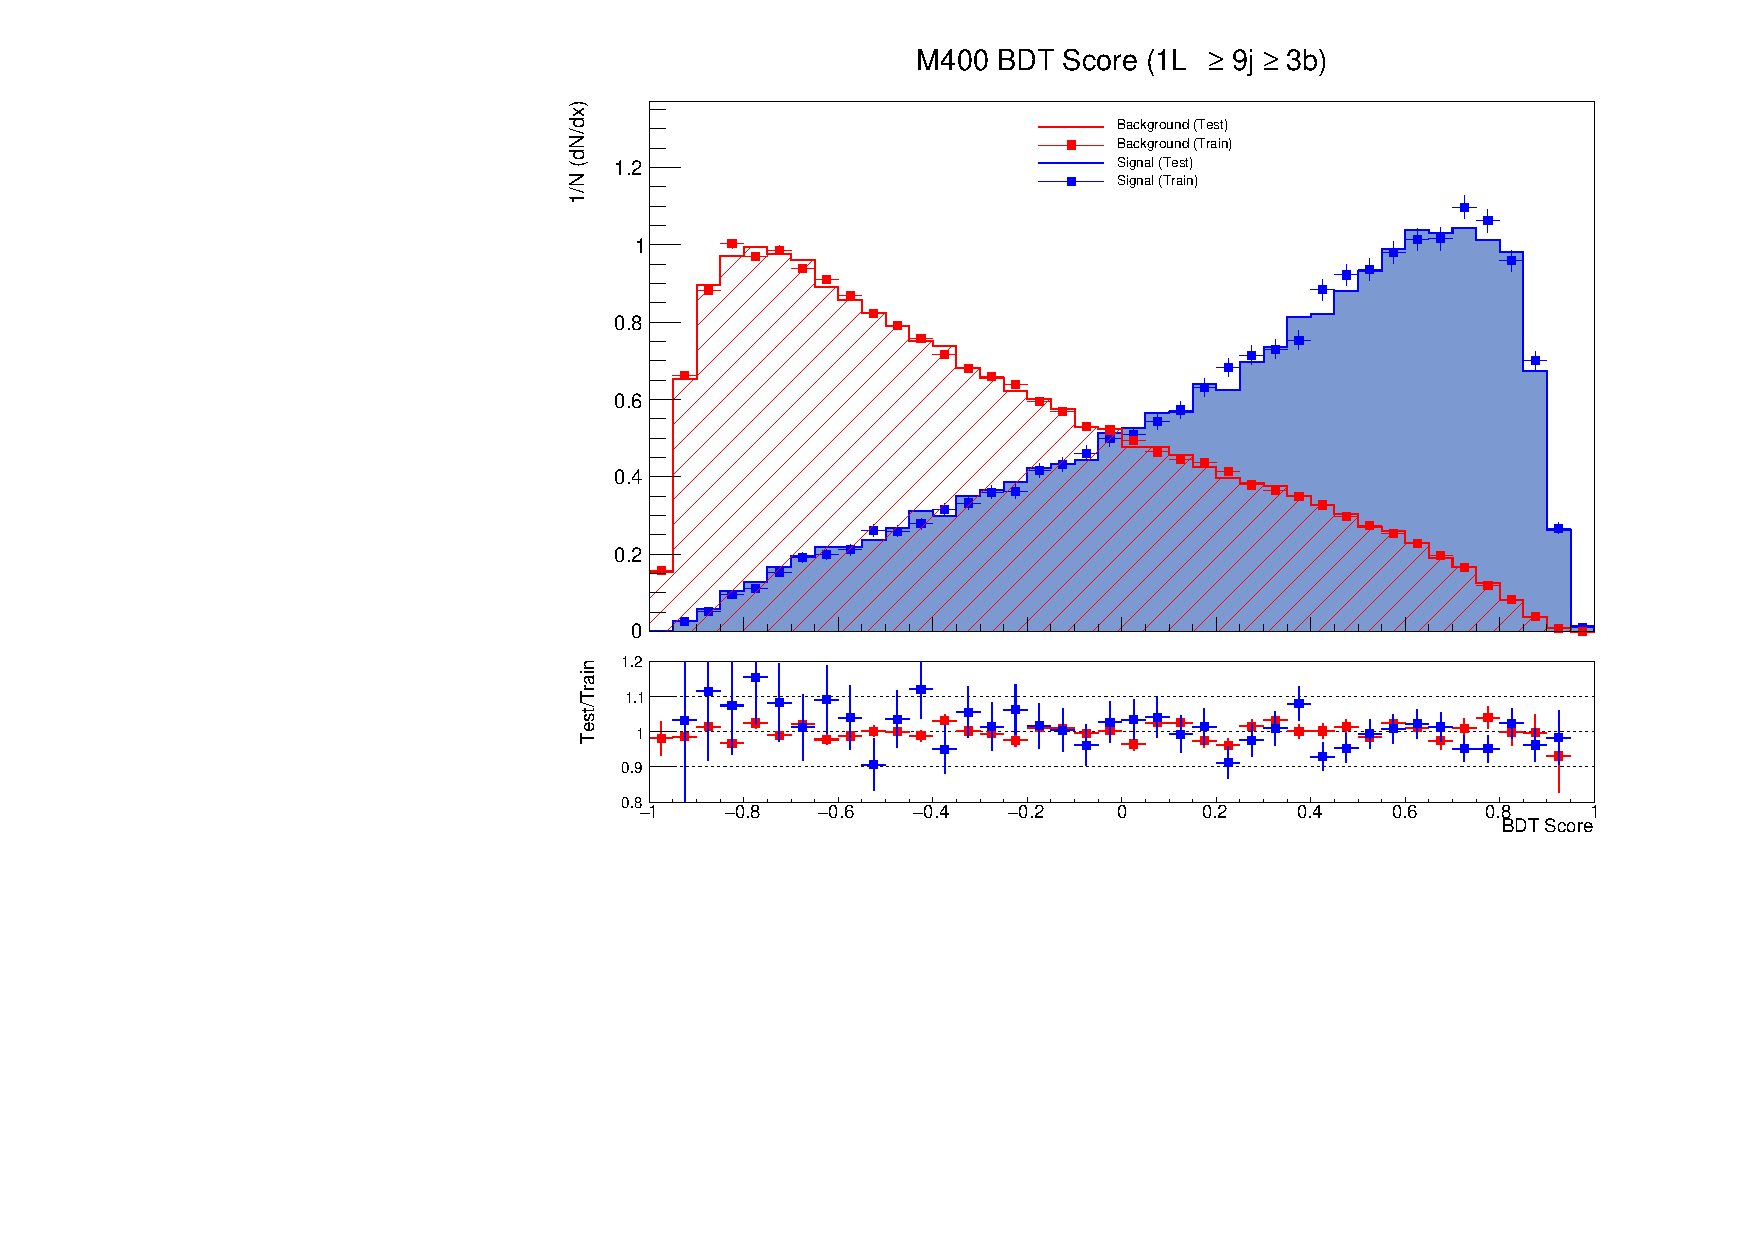
\includegraphics[width=\textwidth]{BDTScore/M400_BDT_1Lge9jge3b.pdf}
        \subcaption{M400 BDT}
    \end{subfigure}
   \begin{subfigure}[t]{0.49\textwidth}
        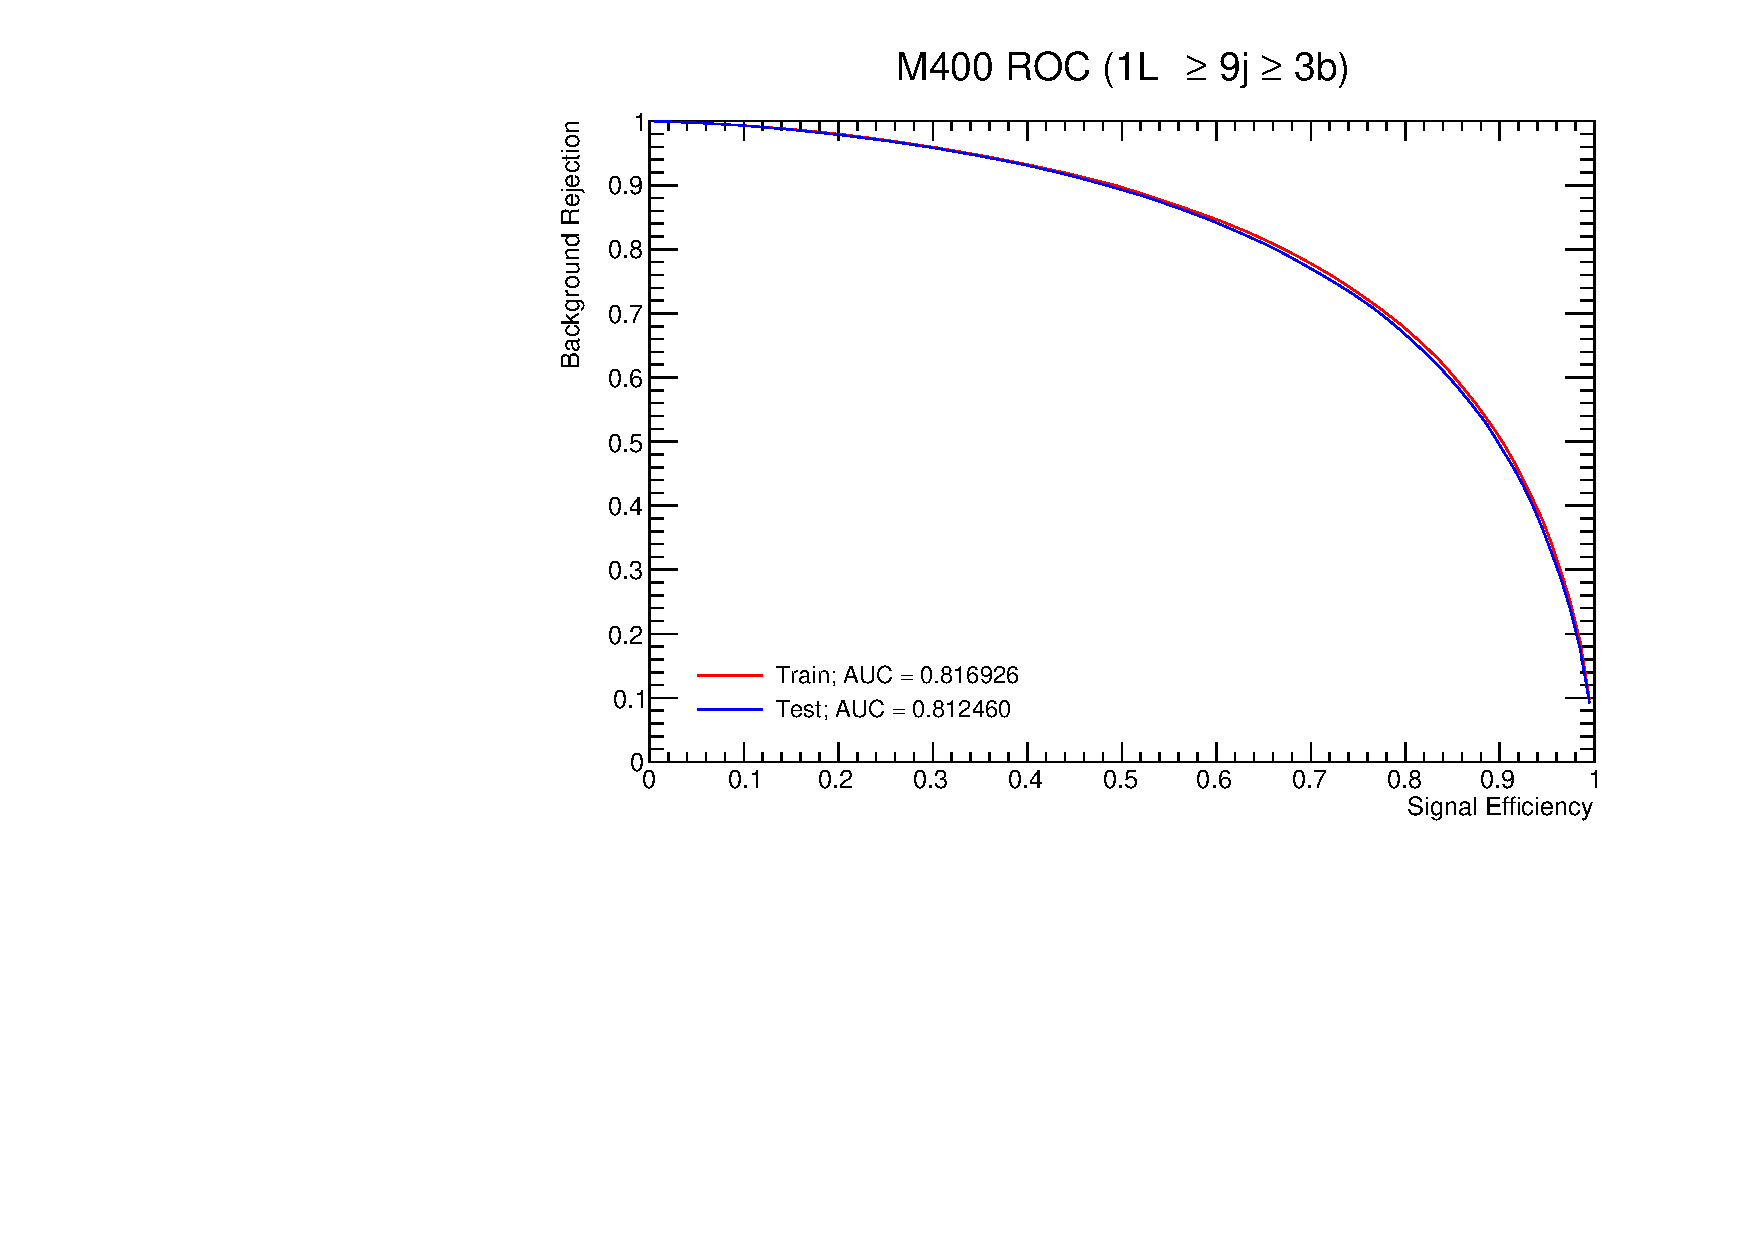
\includegraphics[width=\textwidth]{ROC/M400_ROC_1Lge9jge3b.pdf}
        \subcaption{M400 BDT - ROC}
    \end{subfigure}
    \begin{subfigure}[t]{0.49\textwidth}
        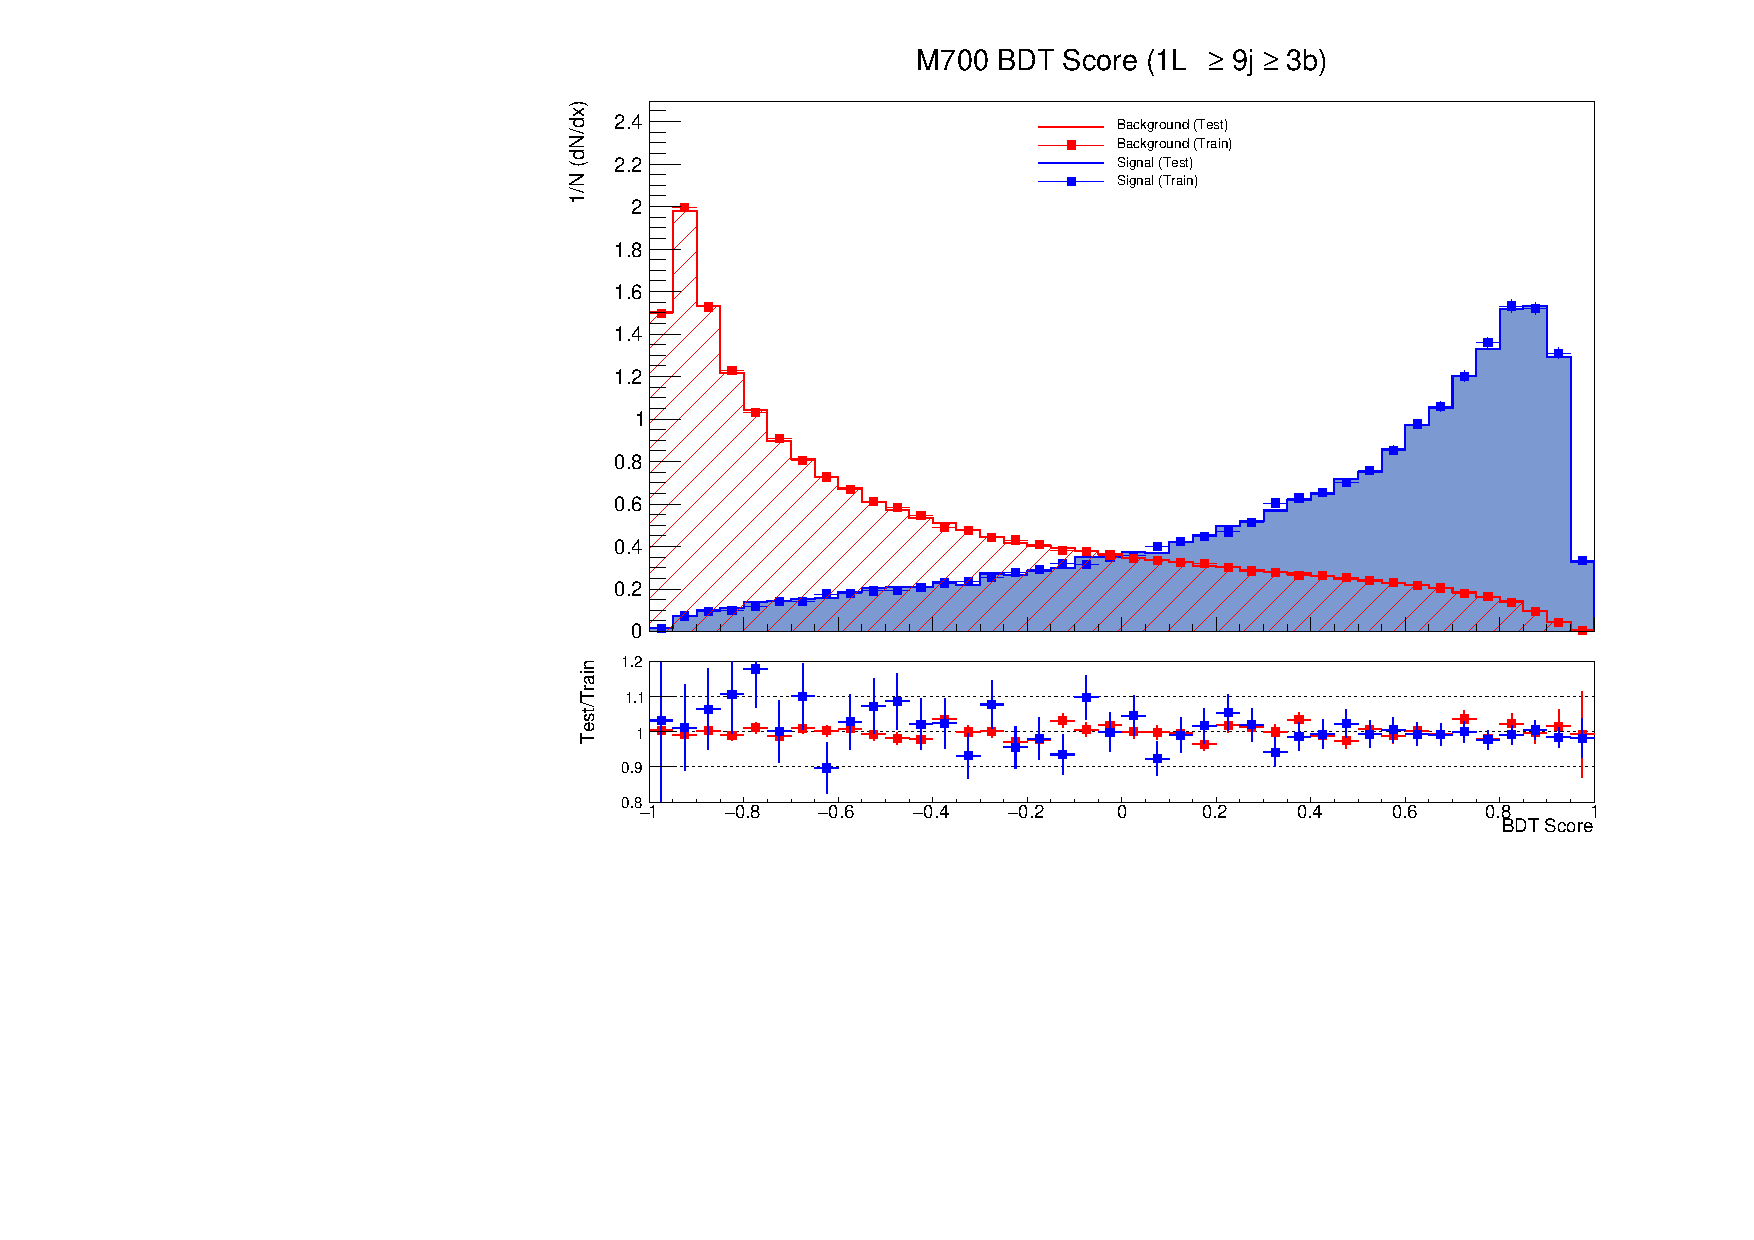
\includegraphics[width=\textwidth]{BDTScore/M700_BDT_1Lge9jge3b.pdf}
        \subcaption{M700 BDT}
    \end{subfigure}
     \begin{subfigure}[t]{0.49\textwidth}
        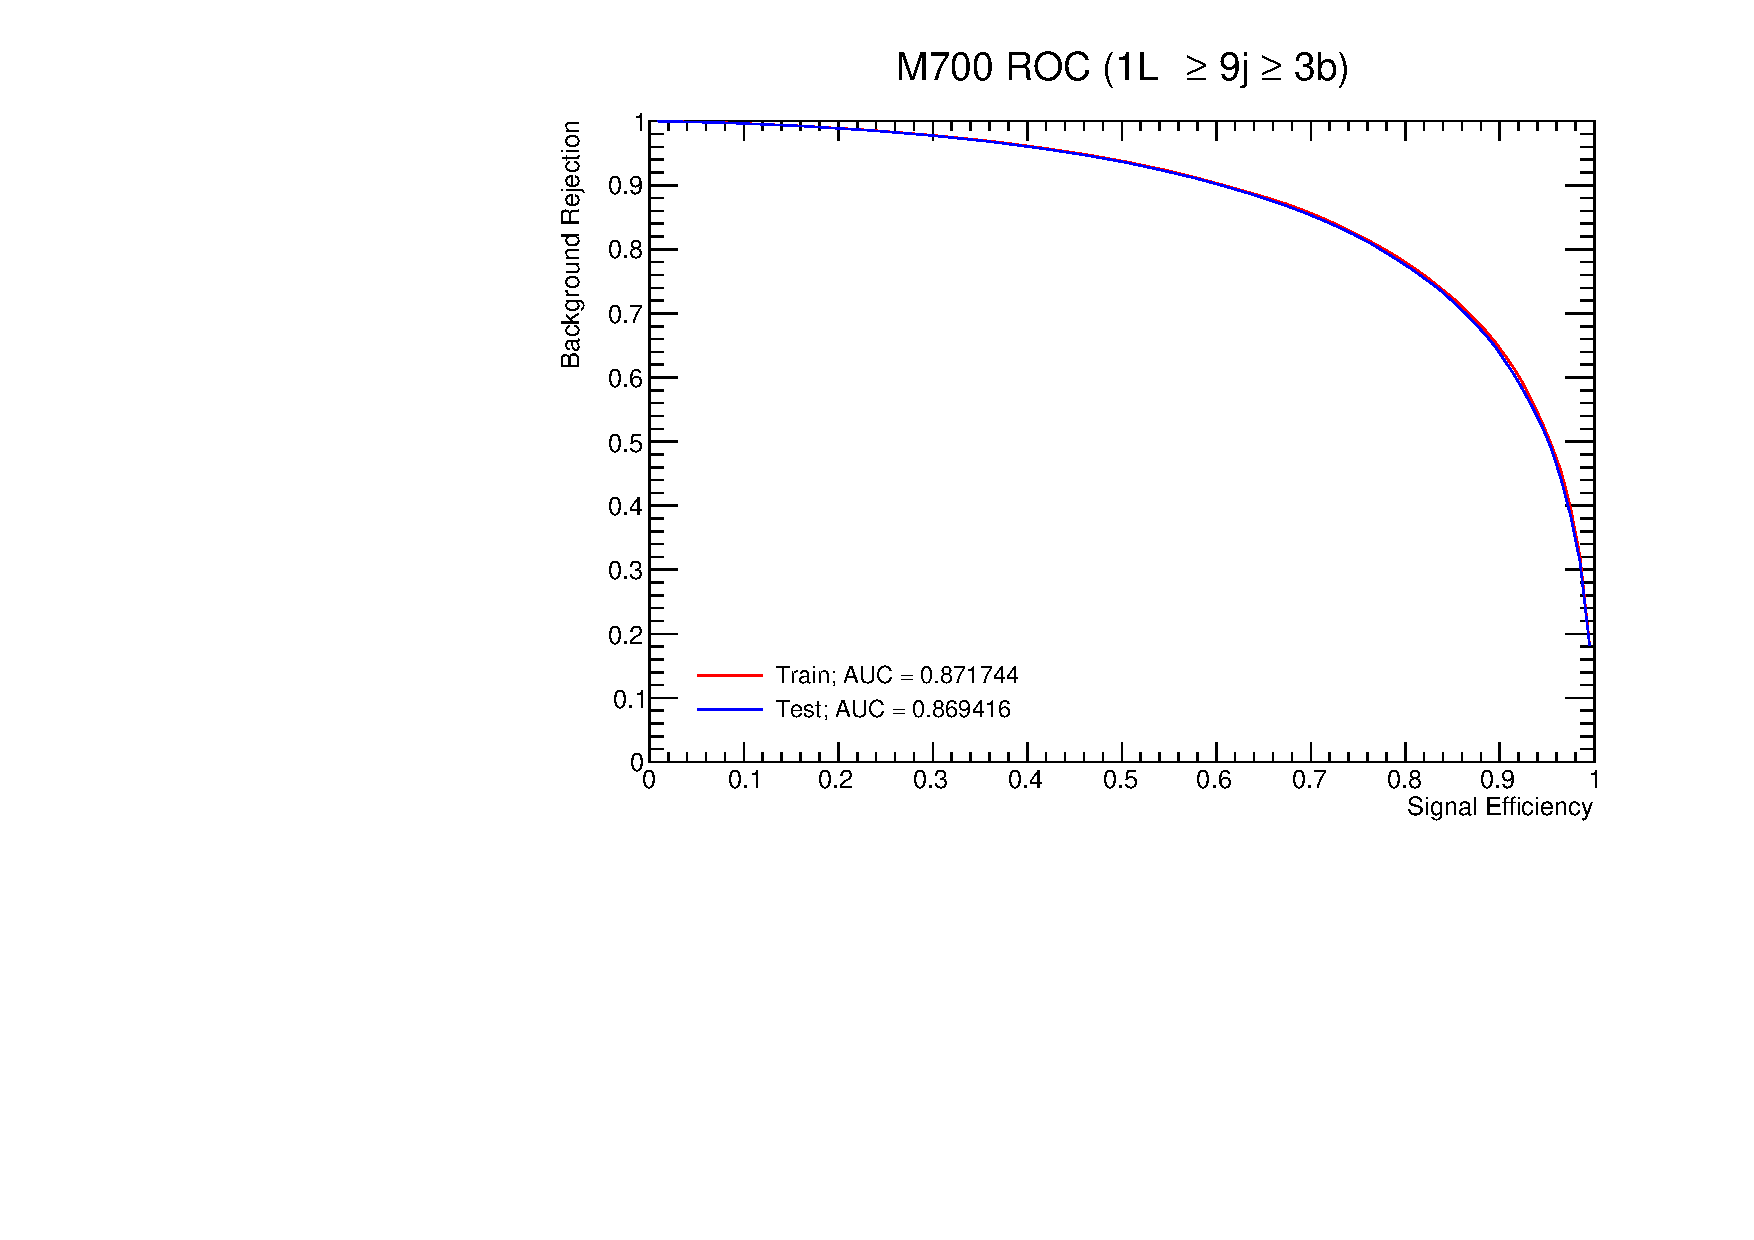
\includegraphics[width=\textwidth]{ROC/M700_ROC_1Lge9jge3b.pdf}
        \subcaption{M700 BDT}
    \end{subfigure}
    \begin{subfigure}[t]{0.49\textwidth}
        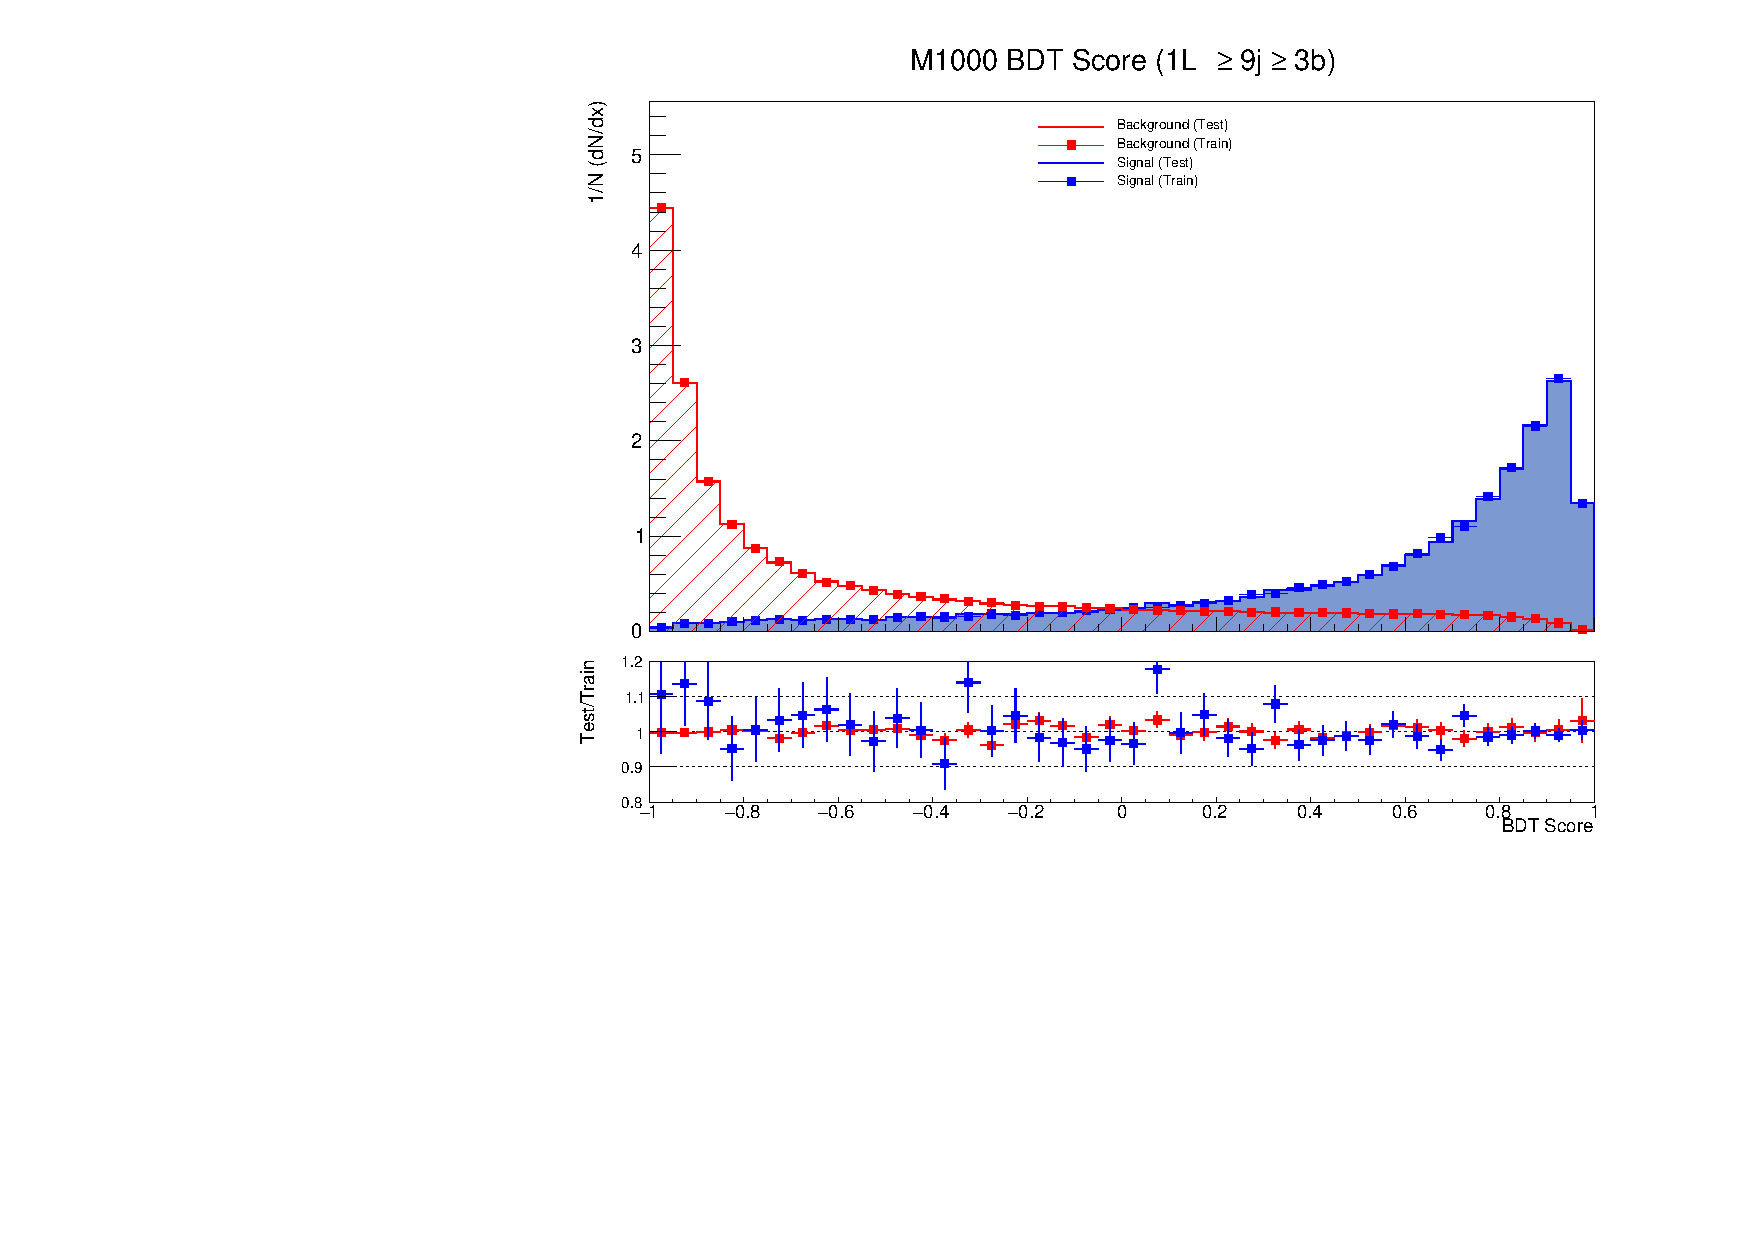
\includegraphics[width=\textwidth]{BDTScore/M1000_BDT_1Lge9jge3b.pdf}
        \subcaption{M1000 BDT}
     \end{subfigure}
     \begin{subfigure}[t]{0.49\textwidth}
        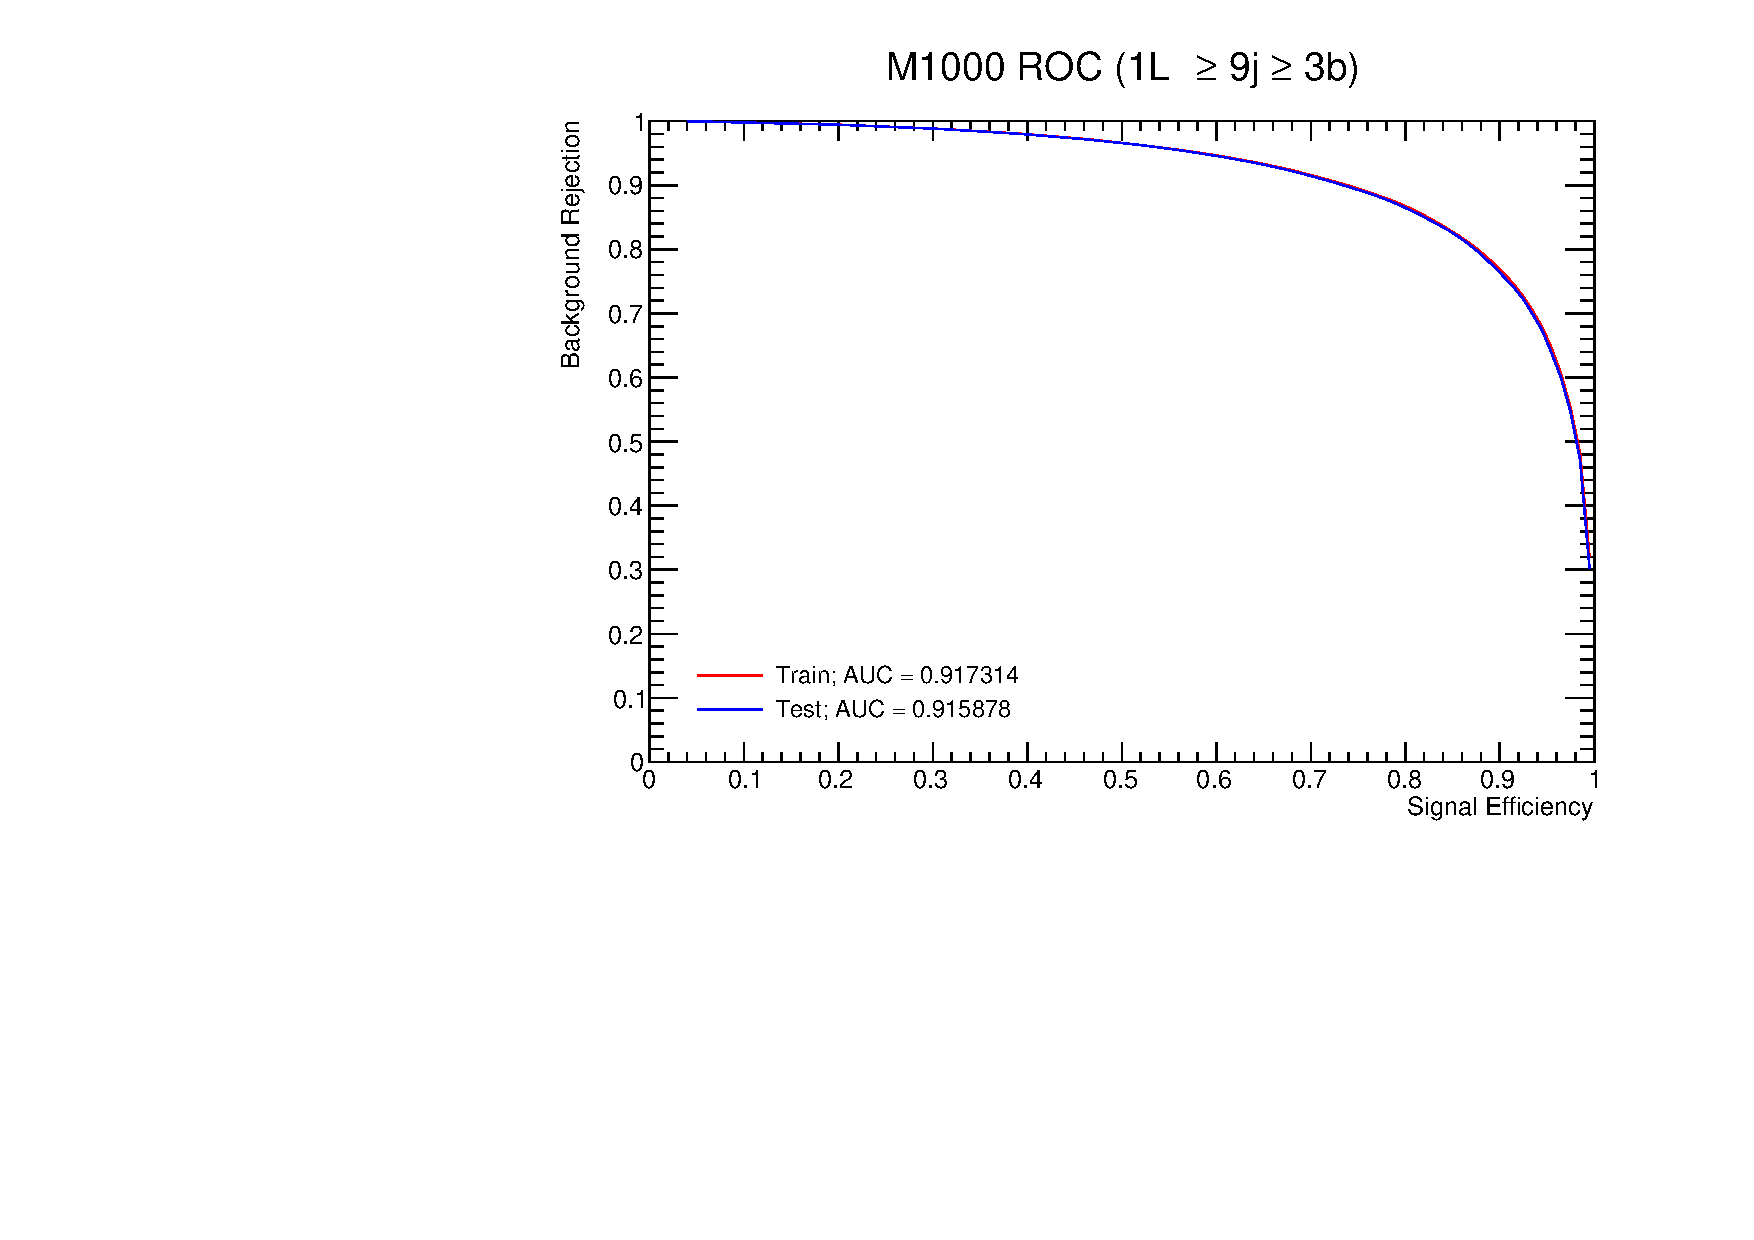
\includegraphics[width=\textwidth]{ROC/M1000_ROC_1Lge9jge3b.pdf}
        \subcaption{M1000 BDT}
    \end{subfigure}
\caption{\label{fig:1Lge9jge3bBDT} Figures in the left show both the training and testing BDT distribution between signal mass points at(a) $400~GeV$, (b) $700~GeV$ and (c) $1000~GeV$ and the $t\bar{t}+$jets background. Figures in the right show the ROC from both training and testing BDT. The region is in 1L$\geq 9j \geq 3b$.}
\end{figure}

\begin{figure}[!htp]\centering
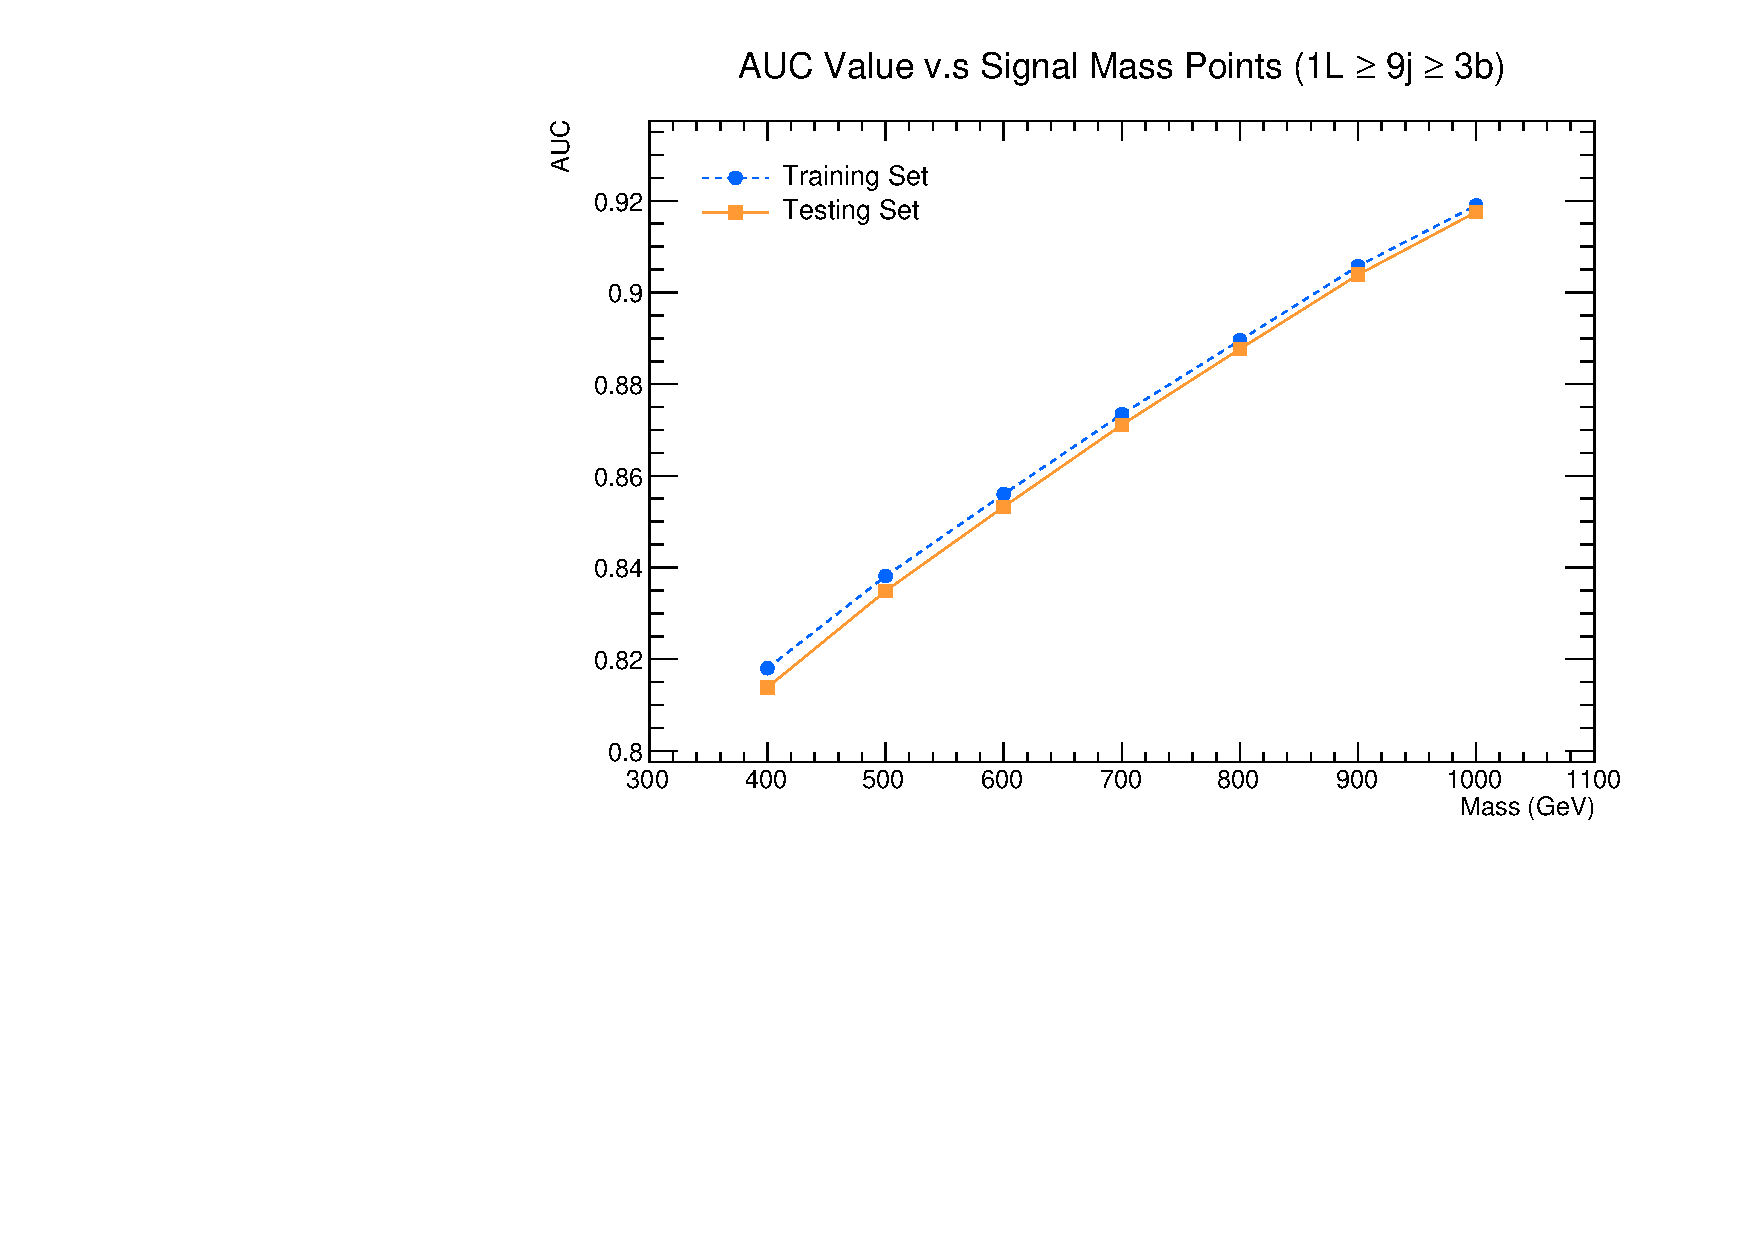
\includegraphics[width=0.45\textwidth]{AUC_perMP_1Lge9jge3b.pdf}
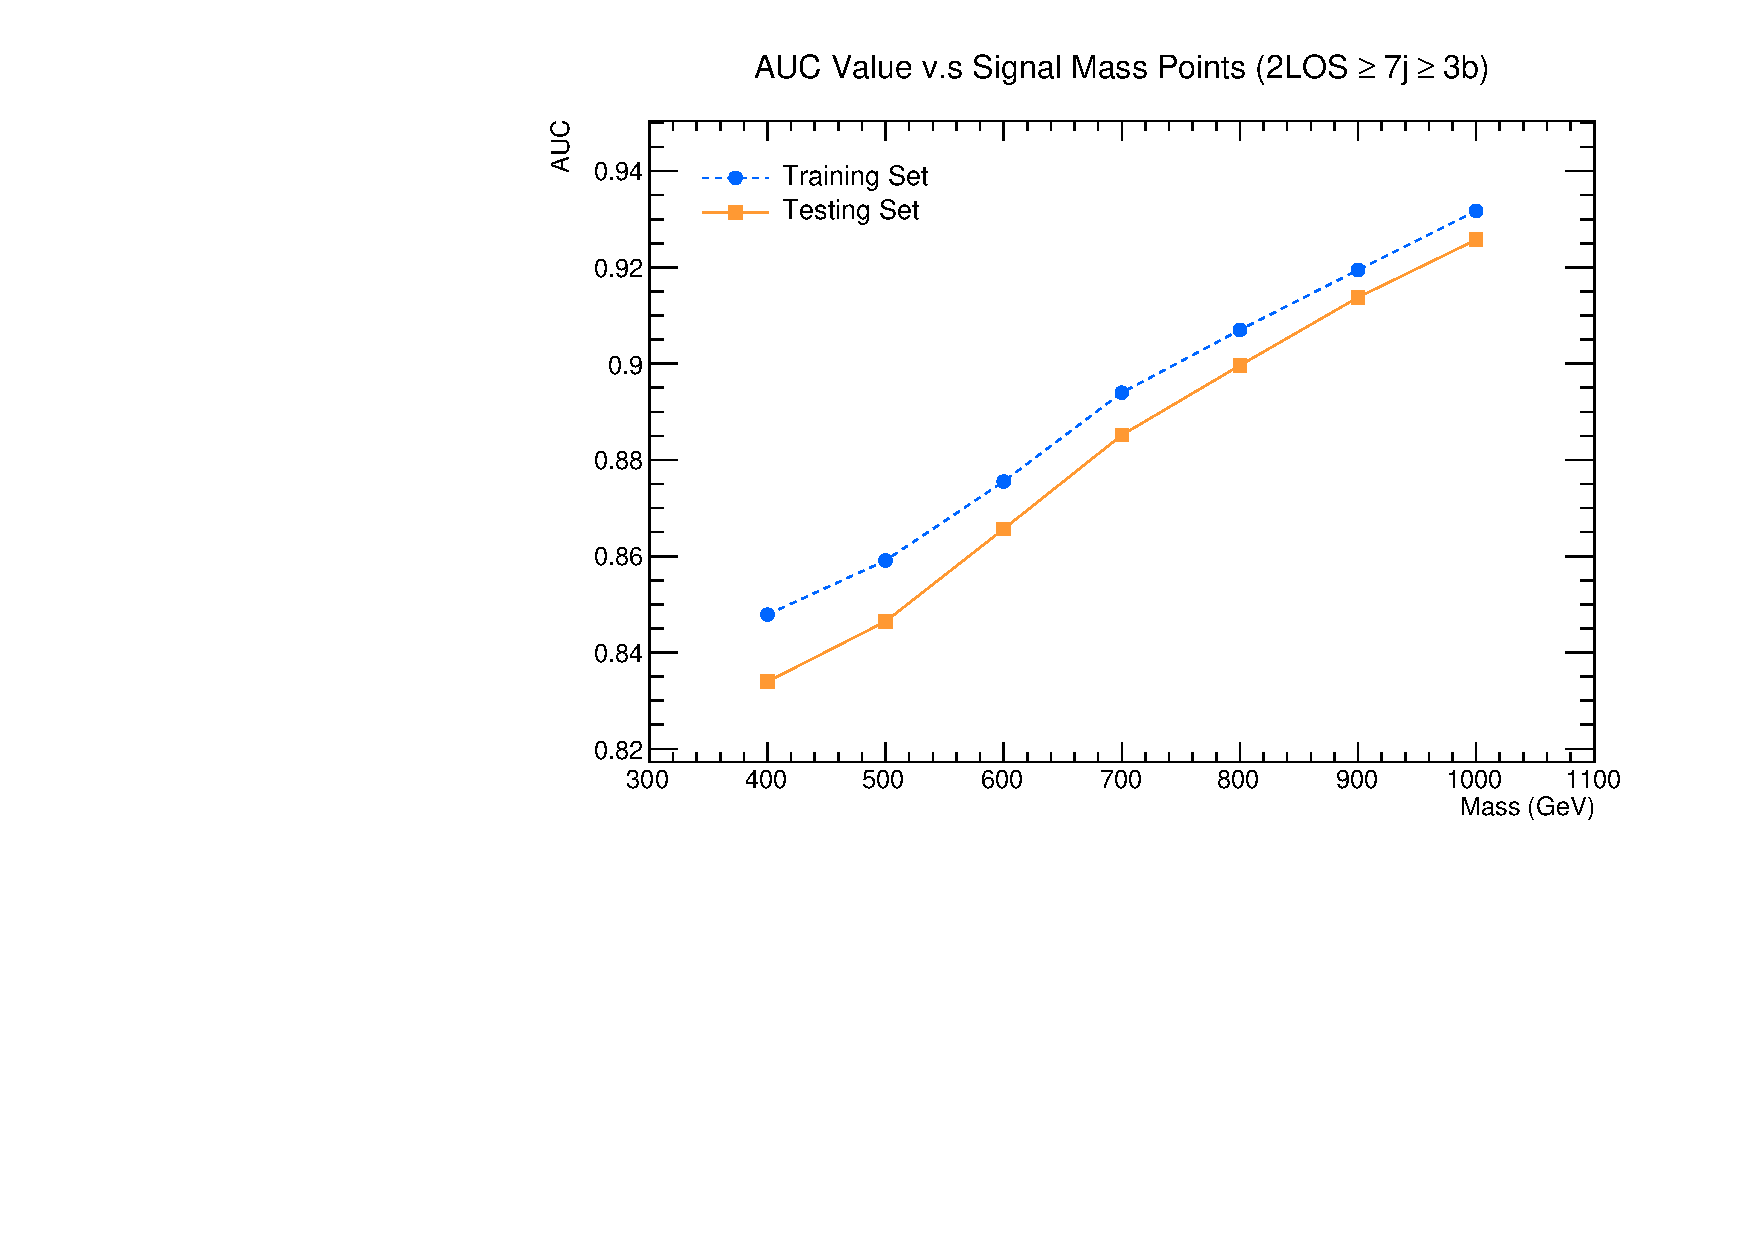
\includegraphics[width=0.45\textwidth]{AUC_perMP_2LOSge7jge3b.pdf}
\caption{\label{fig:AUC_perMP} Plots of AUC value from both training and testing samples against the studying signal mass points from $400~GeV$ to $1000~GeV$ in 1L$\geq 9j \geq 3b$ (left) and 2LOS$\geq 7j \geq 3b$(right).}
\end{figure}
